\documentclass{beamer}

%\usepackage{fontspec}
\usepackage{booktabs}
\usepackage[ngerman]{babel}
\usepackage{verbatim}
\usepackage{fancyvrb}
\usepackage{listings}
\usepackage{csquotes}
\usepackage[style=authoryear]{biblatex} 
\usepackage{graphicx}

\usepackage{hyperref}
\usepackage{amsmath,amssymb}
\newcommand\Z{\ensuremath{\mathbb{Z}}}
\newcommand\N{\ensuremath{\mathbb{N}}}
\newcommand\Q{\ensuremath{\mathbb{Q}}}
\usepackage[ngerman]{babel}
\usepackage{csquotes}

\usepackage{pdfpages}

\usepackage{float}


\usepackage{biblatex}
\addbibresource{../../../zotero.bib}

\title{Parametrisches Design, dadurch entstehende Bauweisen und Topologie in Produktdesign und Architektur}  
\author{Daniel Renschler}
\date{6. Oktober 2023}

\usetheme{Frankfurt}
\usecolortheme{crane}

\begin{document}

\begin{frame}
    \titlepage 
\end{frame}


\section{Einleitung}
\begin{frame}{These}
Design\footnote{Design als Architektur und Produktdesign, nicht z.B.
Grafikdesign.} hatte noch keine Digitale Revolution.

\begin{itemize}
    \item In den nächsten 15 Jahren wird sich das ändern.

    \item Aber nicht mit K.I. wie in \parencite{oppenlaender2022}, sondern mit
        Algorithmen\footnote{Eindeutige Handlungsvorschrift zur Lösung
        eines Problems oder einer Klasse von Problemen}
\end{itemize}
\end{frame}


\begin{frame}{Status Quo}
   \begin{itemize}
       \item Designer Arbeiten mit Programmen
       \item Computer sind aber kein partizipierender Akteur im Prozess
   \end{itemize} 
\end{frame}


\begin{frame}
    \tableofcontents
\end{frame}

\begin{frame}{Mies Van der Rohe \"uber Technologie}
    \begin{quote}
        Wherever technology reaches its real fulfillment, it transcends into architecture.
    \end{quote}
\end{frame}


\section{Begriffe}
\begin{frame}{Was ist Parametrisches Design?}
    \begin{itemize}
        \item Design erstellt oder erzeugt nach Parametern und Regeln
        \item Meist Algorithmisch
        \item Auch durch Mathematische Optimierungen
    \end{itemize}
\end{frame}



\begin{frame}{Was ist Topologie?}
    \begin{itemize}
        \item Abstraktes Teilgebiet der Mathematik
            \begin{itemize}
                \item Mengenlehre
                \item Anordnung geometrischer Gebilde im Raum
                \item Geometrie 
            \end{itemize}
        \item Zu unseren Zwecken nur in $x\in \N$ Dimensionen
    \end{itemize}
\end{frame}

\begin{frame}{Was ist Topologie? 2}
\begin{figure}[htpb]
    \centering
    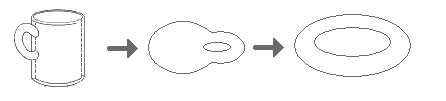
\includegraphics[width=0.8\textwidth]{figures/Homeo_tasse.png}
    \caption{Homeo Tasse}
    \label{fig:Homeo Tasse}
\end{figure}
\end{frame}

    
\section{Topologie}
\begin{frame}{Topologische Optimierungen}
    \begin{figure}[htbp]
        \begin{minipage}{0.2\textwidth}
            \centering
            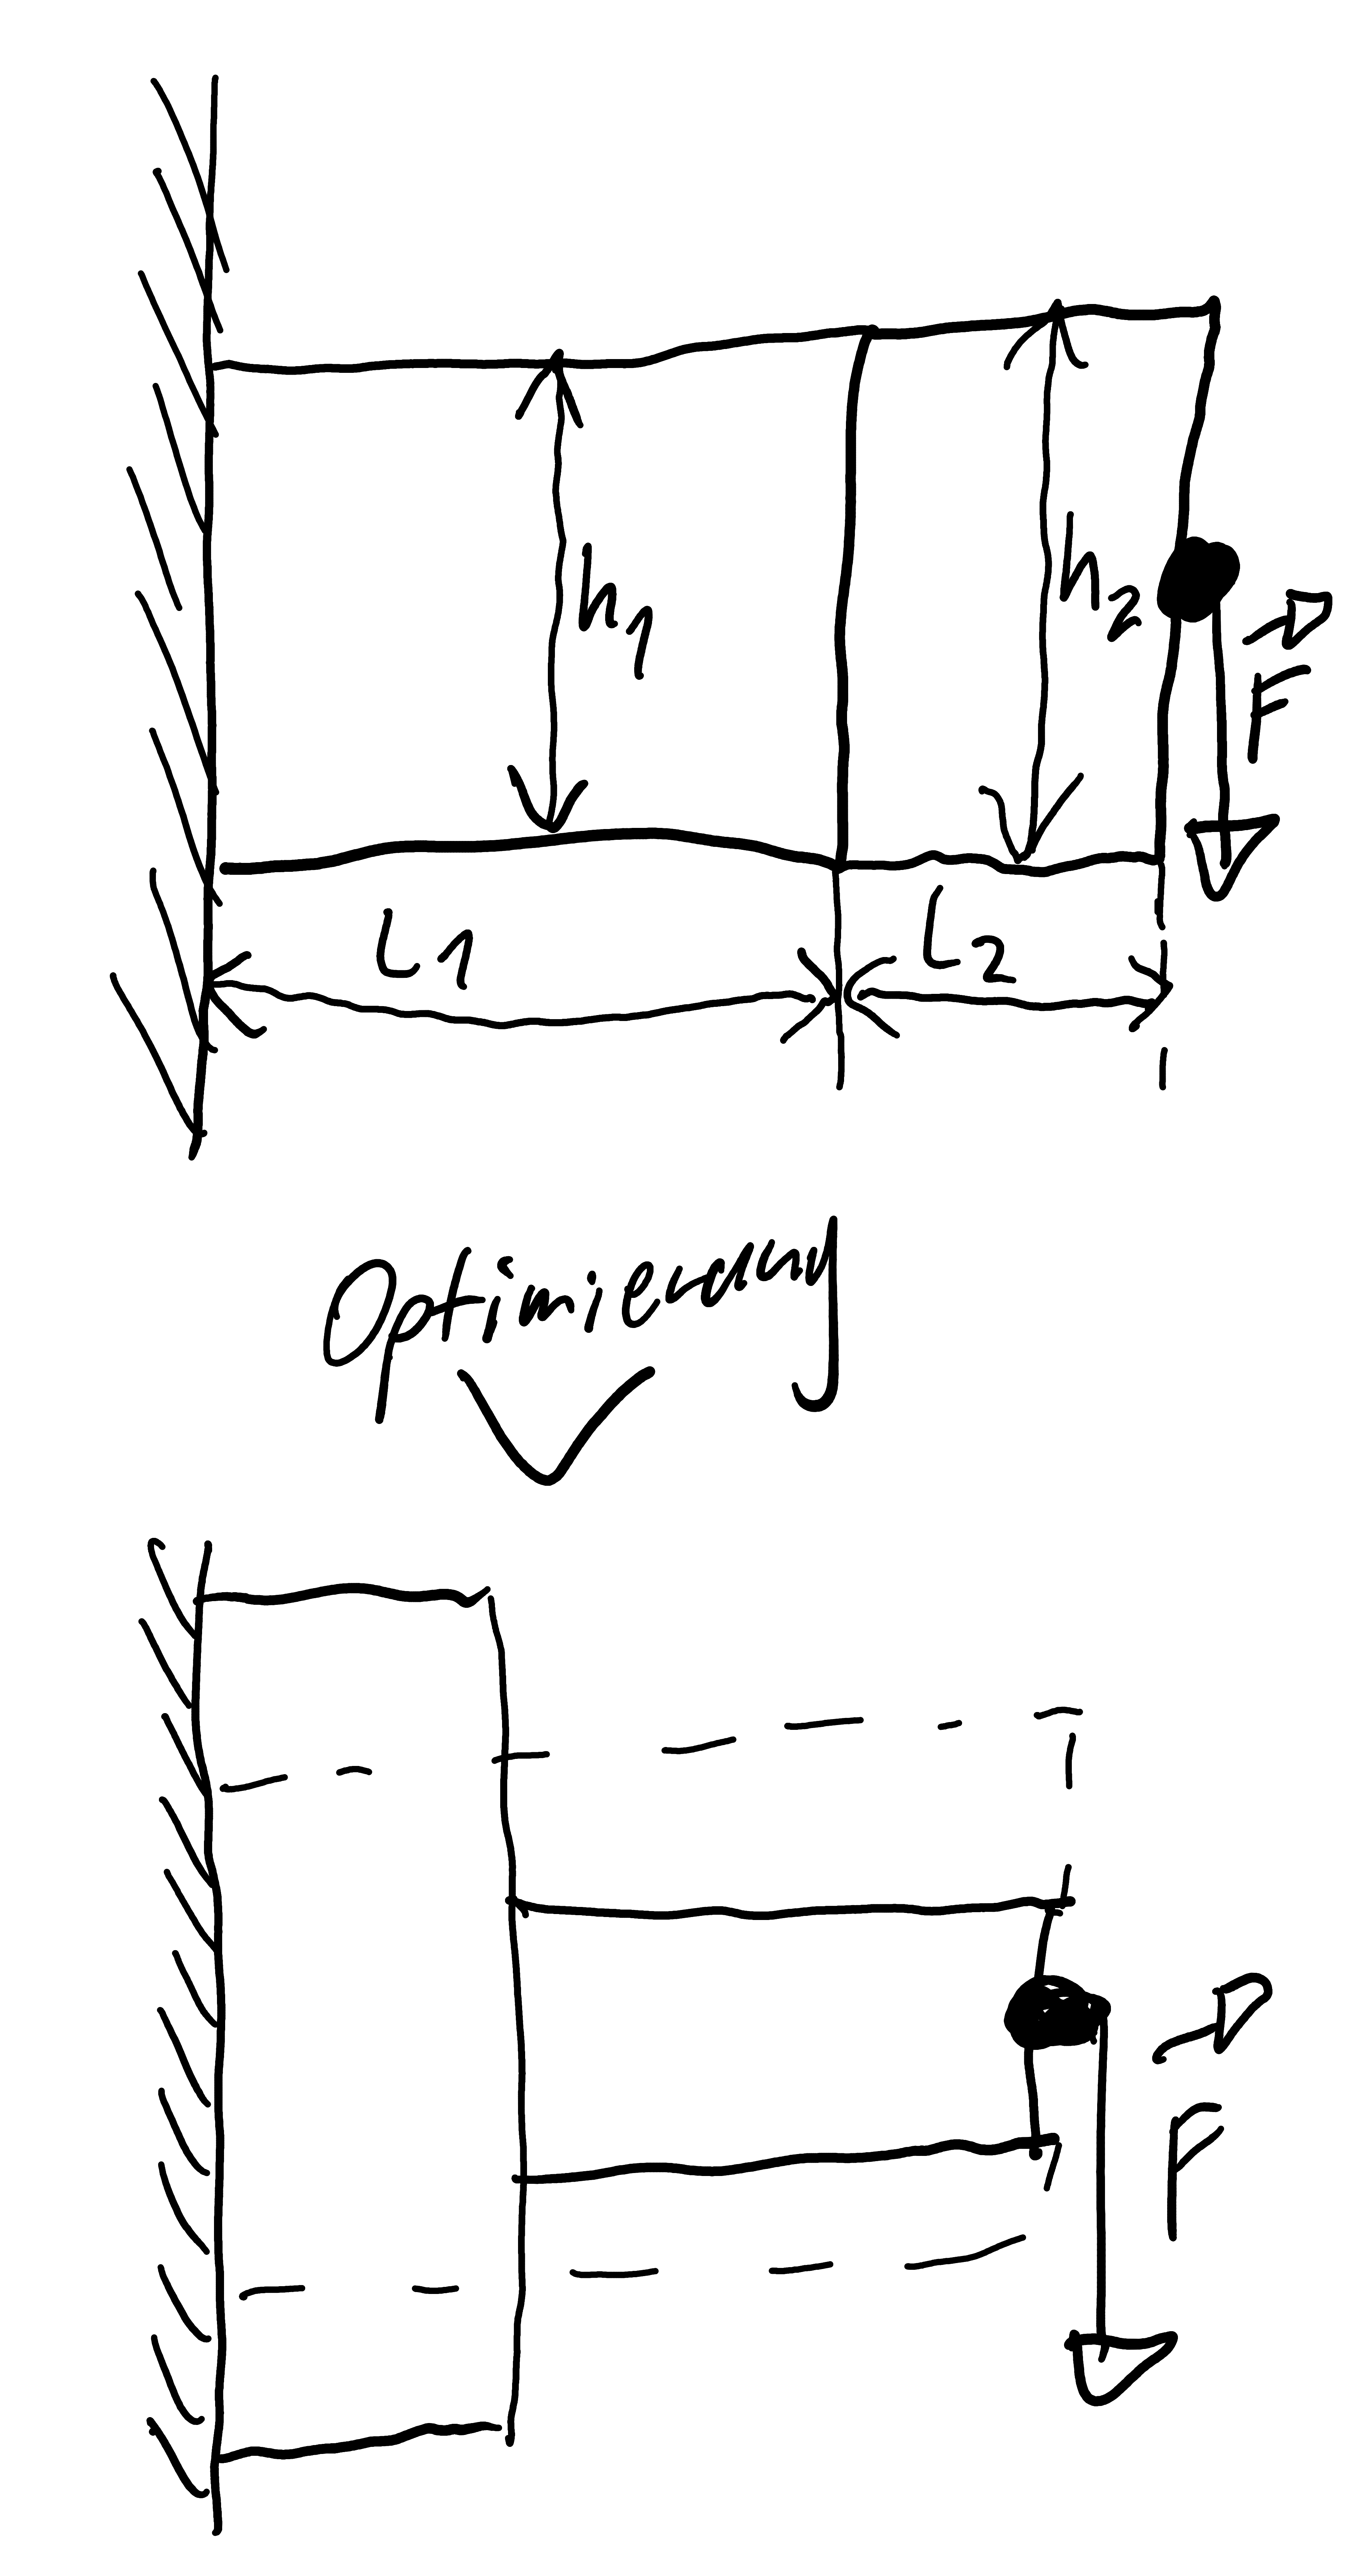
\includegraphics[width=\linewidth]{figures/Groesen-opt.png}
            \caption{Gr\"o\ss{}en Optimierung}
        \end{minipage}\hfill
        \begin{minipage}{0.2\textwidth}
            \centering
            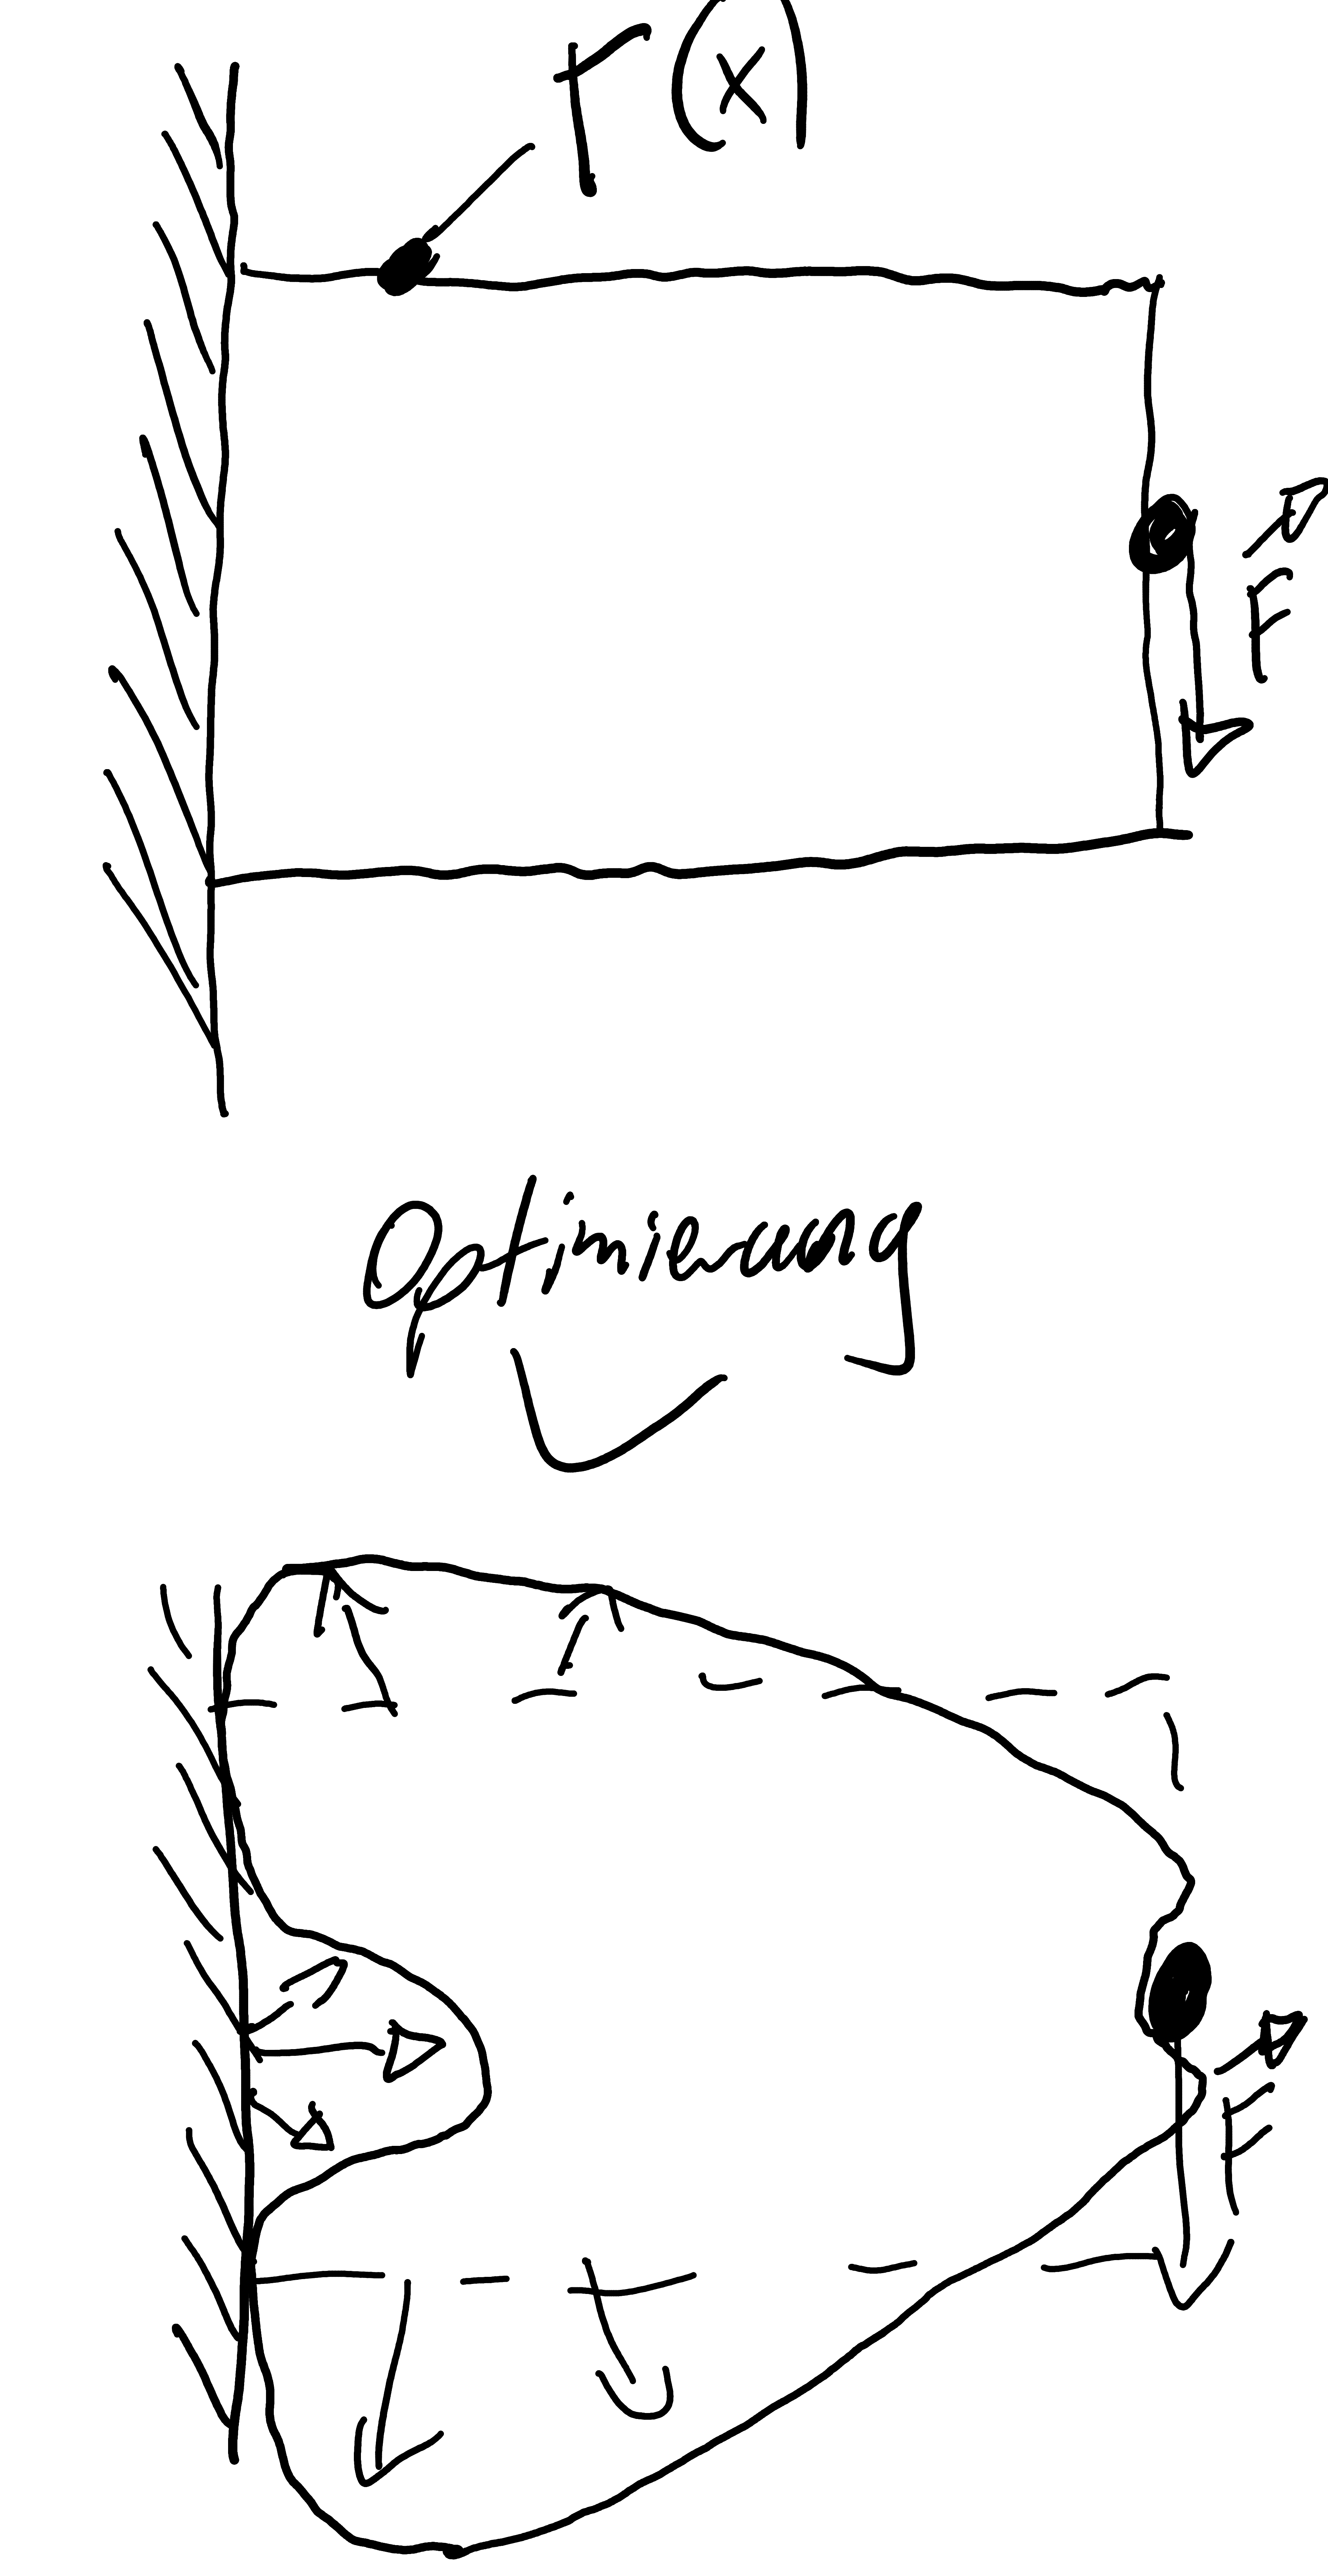
\includegraphics[width=\linewidth]{figures/Form-opt.png}
            \caption{Form Optimierung}
        \end{minipage}\hfill
        \begin{minipage}{0.2\textwidth}
            \centering
            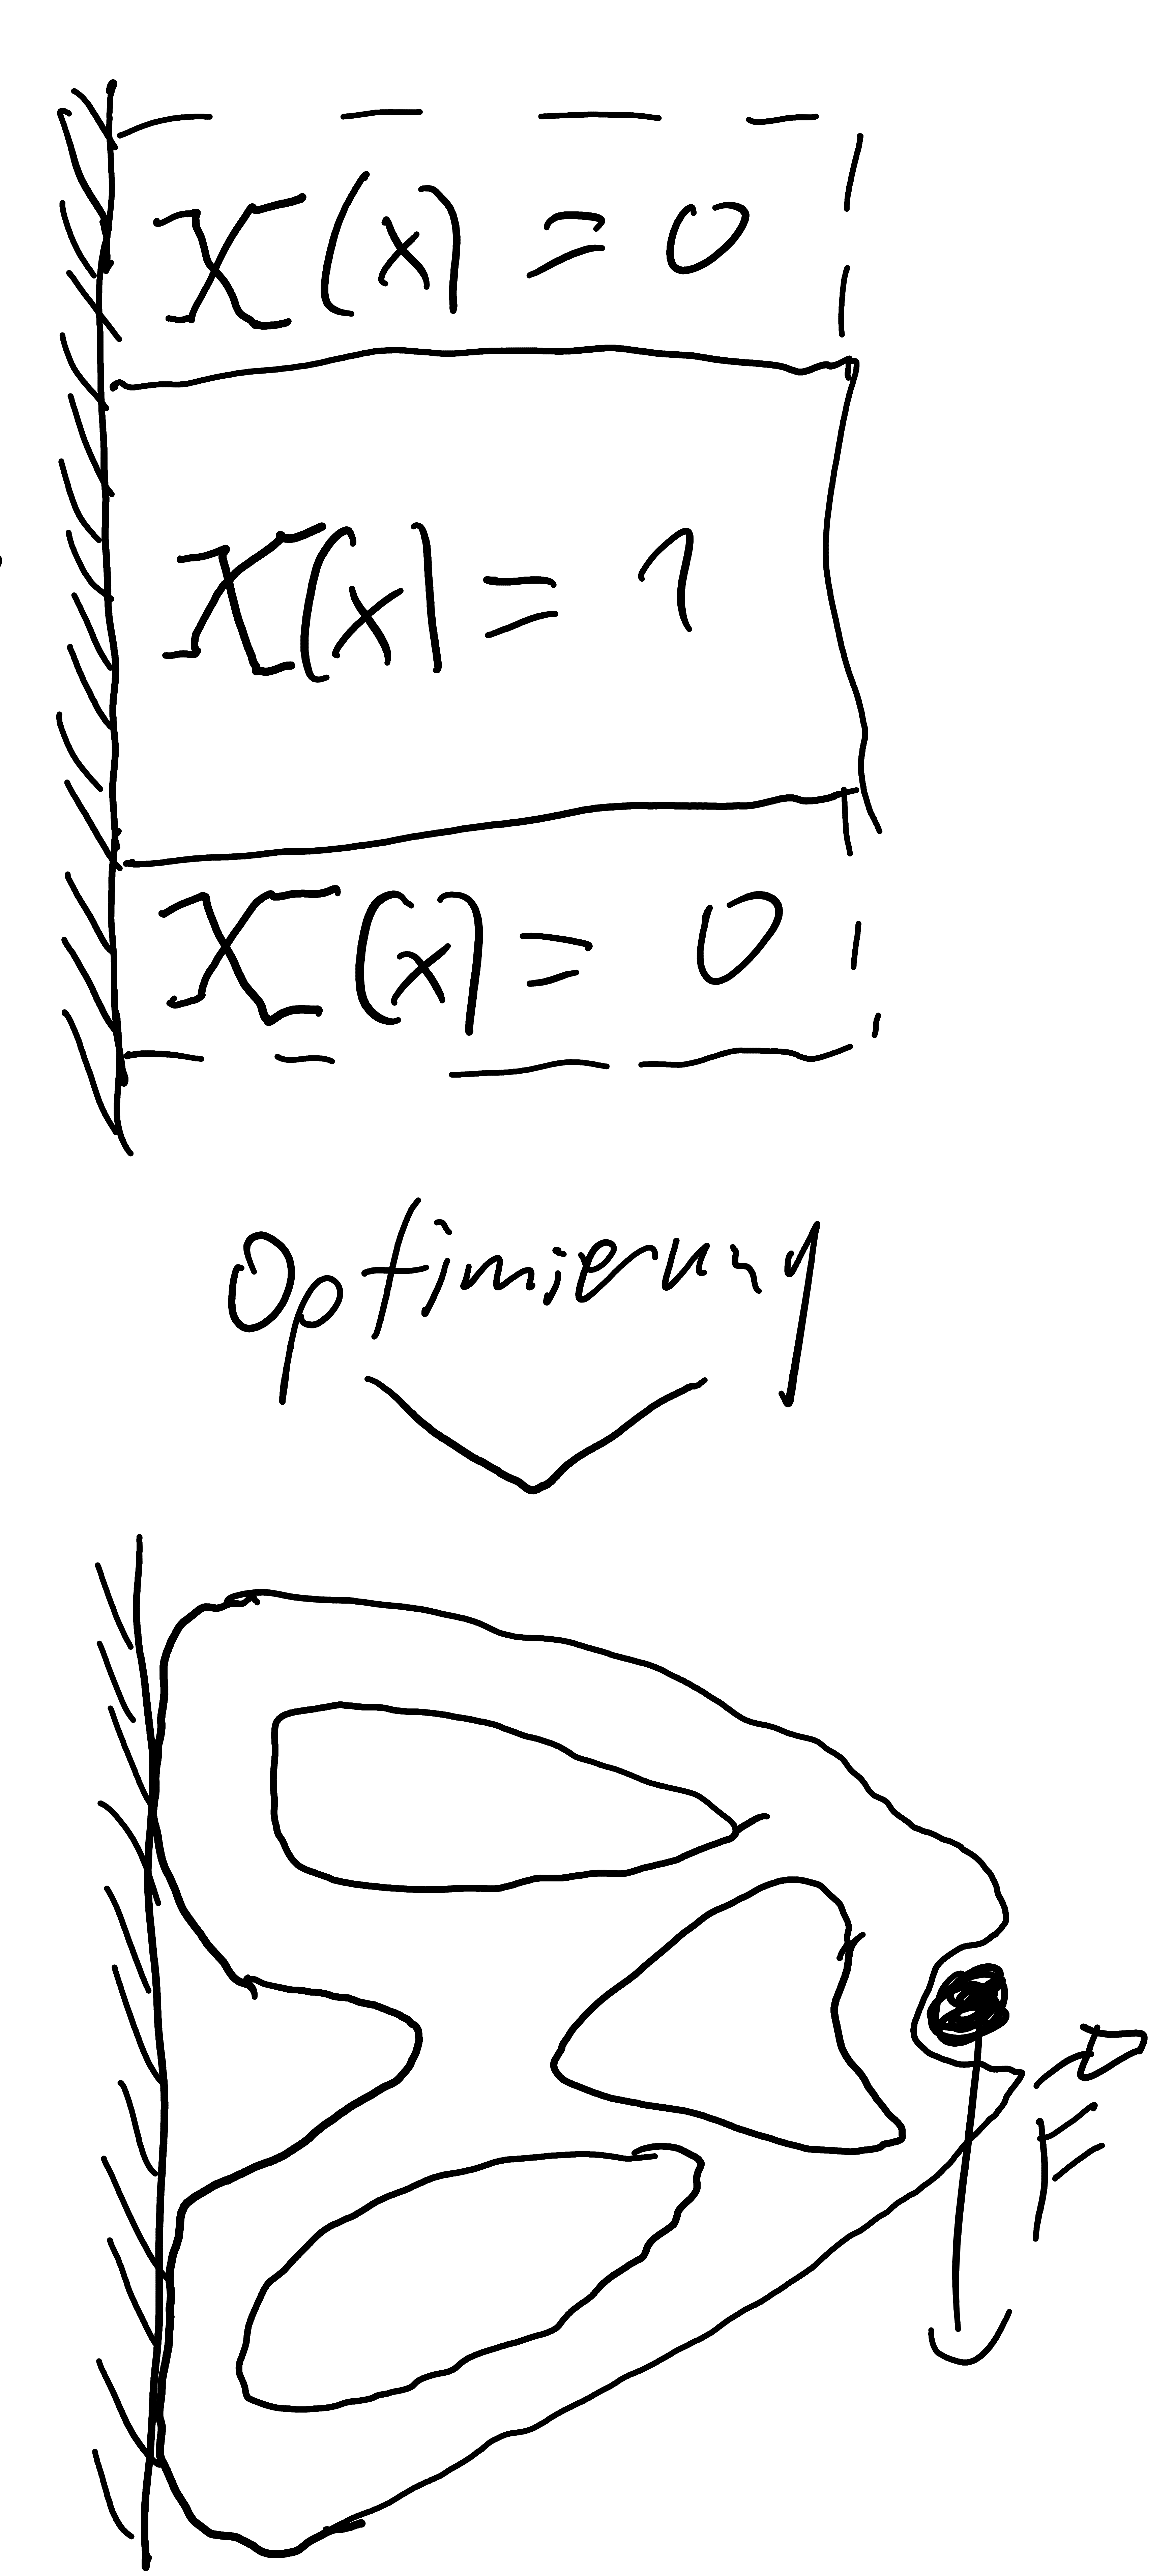
\includegraphics[width=\linewidth]{figures/Topo-opt.png}
            \caption{Topologische Optimierung}
        \end{minipage}
        \caption{Unterschied zwischen verschiedenen Optimierungen}
        \label{fig:unterschied}
    \end{figure}
\end{frame}



\begin{frame}{Topologie Rechnen}
\begin{equation}
    c=\frac{1}{2}U^{T}K\cdot \vec{U}
\end{equation}

\begin{enumerate}
    \item $c$ = Kostenma\ss
    \item $\vec{U}$ = Verschiebung und Deformation in einem System
    \item $U^T$ = der Vektor aber Transponiert\footnote{transponiert $\approx$ gespiegelt}
    \item $K$ = Steifigkeitsmatrix
\end{enumerate}
\end{frame}



\begin{frame}{Topologie Rechnen 2}
\begin{equation}
    c = \frac{1}{2}fu = \frac{1}{2}ku^2
\end{equation}

\begin{enumerate}
    \item $c$ = elastische Energie
    \item $f$ = auf das System ausge\"ubte Kraft
    \item $k$ = Federkonstante
    \item $u$ = Deformation im System
\end{enumerate}
\end{frame}



\begin{frame}{Topologie Rechnen 3}
    \begin{equation}
        k\vec{u} = f
    \end{equation}
    \begin{enumerate}
        \item $k$ = Steifigkeitsmatrix
        \item $f$ = auf das System ausge\"ubte Kraft
        \item $\vec{u}$ = Verformung im System
    \end{enumerate}
\end{frame}


\begin{frame}{Topologie Rechnen 4}
    Die Gleichungen sind von einigen Bedingungen Abh\"angig:
    \begin{itemize}
    \item $ku = F$: Diese Formulierung repräsentiert die statische
        Gleichgewichtsgleichung, die besagt, dass die resultierende Verformung
        $u$ im System gleich der externen angewandten Kraft $F$ ist. 

    \item $\rho_i \in \{1 \text{ (vorhanden)}, 0 \text{ (leer)}\}, \forall i$: 
        Dies gibt an, dass $\rho_i$ entweder den Wert 1 (vorhanden)
        oder 0 (leer) haben kann. Dabei repräsentiert $i$ die einzelnen
        Elemente des Systems.

    \item $g = \sum_i \rho_i - V_0 \leq 0$: Dies ist die letzte Nebenbedingung,
        die besagt, dass die Summe der $\rho_i$ Werte minus $V_0$ kleiner oder
        gleich null sein muss, wobei $V_0$ eine bestimmte Schwelle für das
        Erscheinen der Elemente im System darstellt.
\end{itemize}
\end{frame}



\begin{frame}{Topologie Simulieren}
Diese Sektion wird sich mit einer Simulations Software \parencite{aage2014} der
Deanmarks Tekniske Universitet besch\"aftigen, diese ist zwei-Dimensional und
gut um Zusammenh\"ange intuitiv zu zeigen.
\end{frame}

\begin{frame}{Topologie Simulieren 2}
\begin{figure}[H]
    \centering
    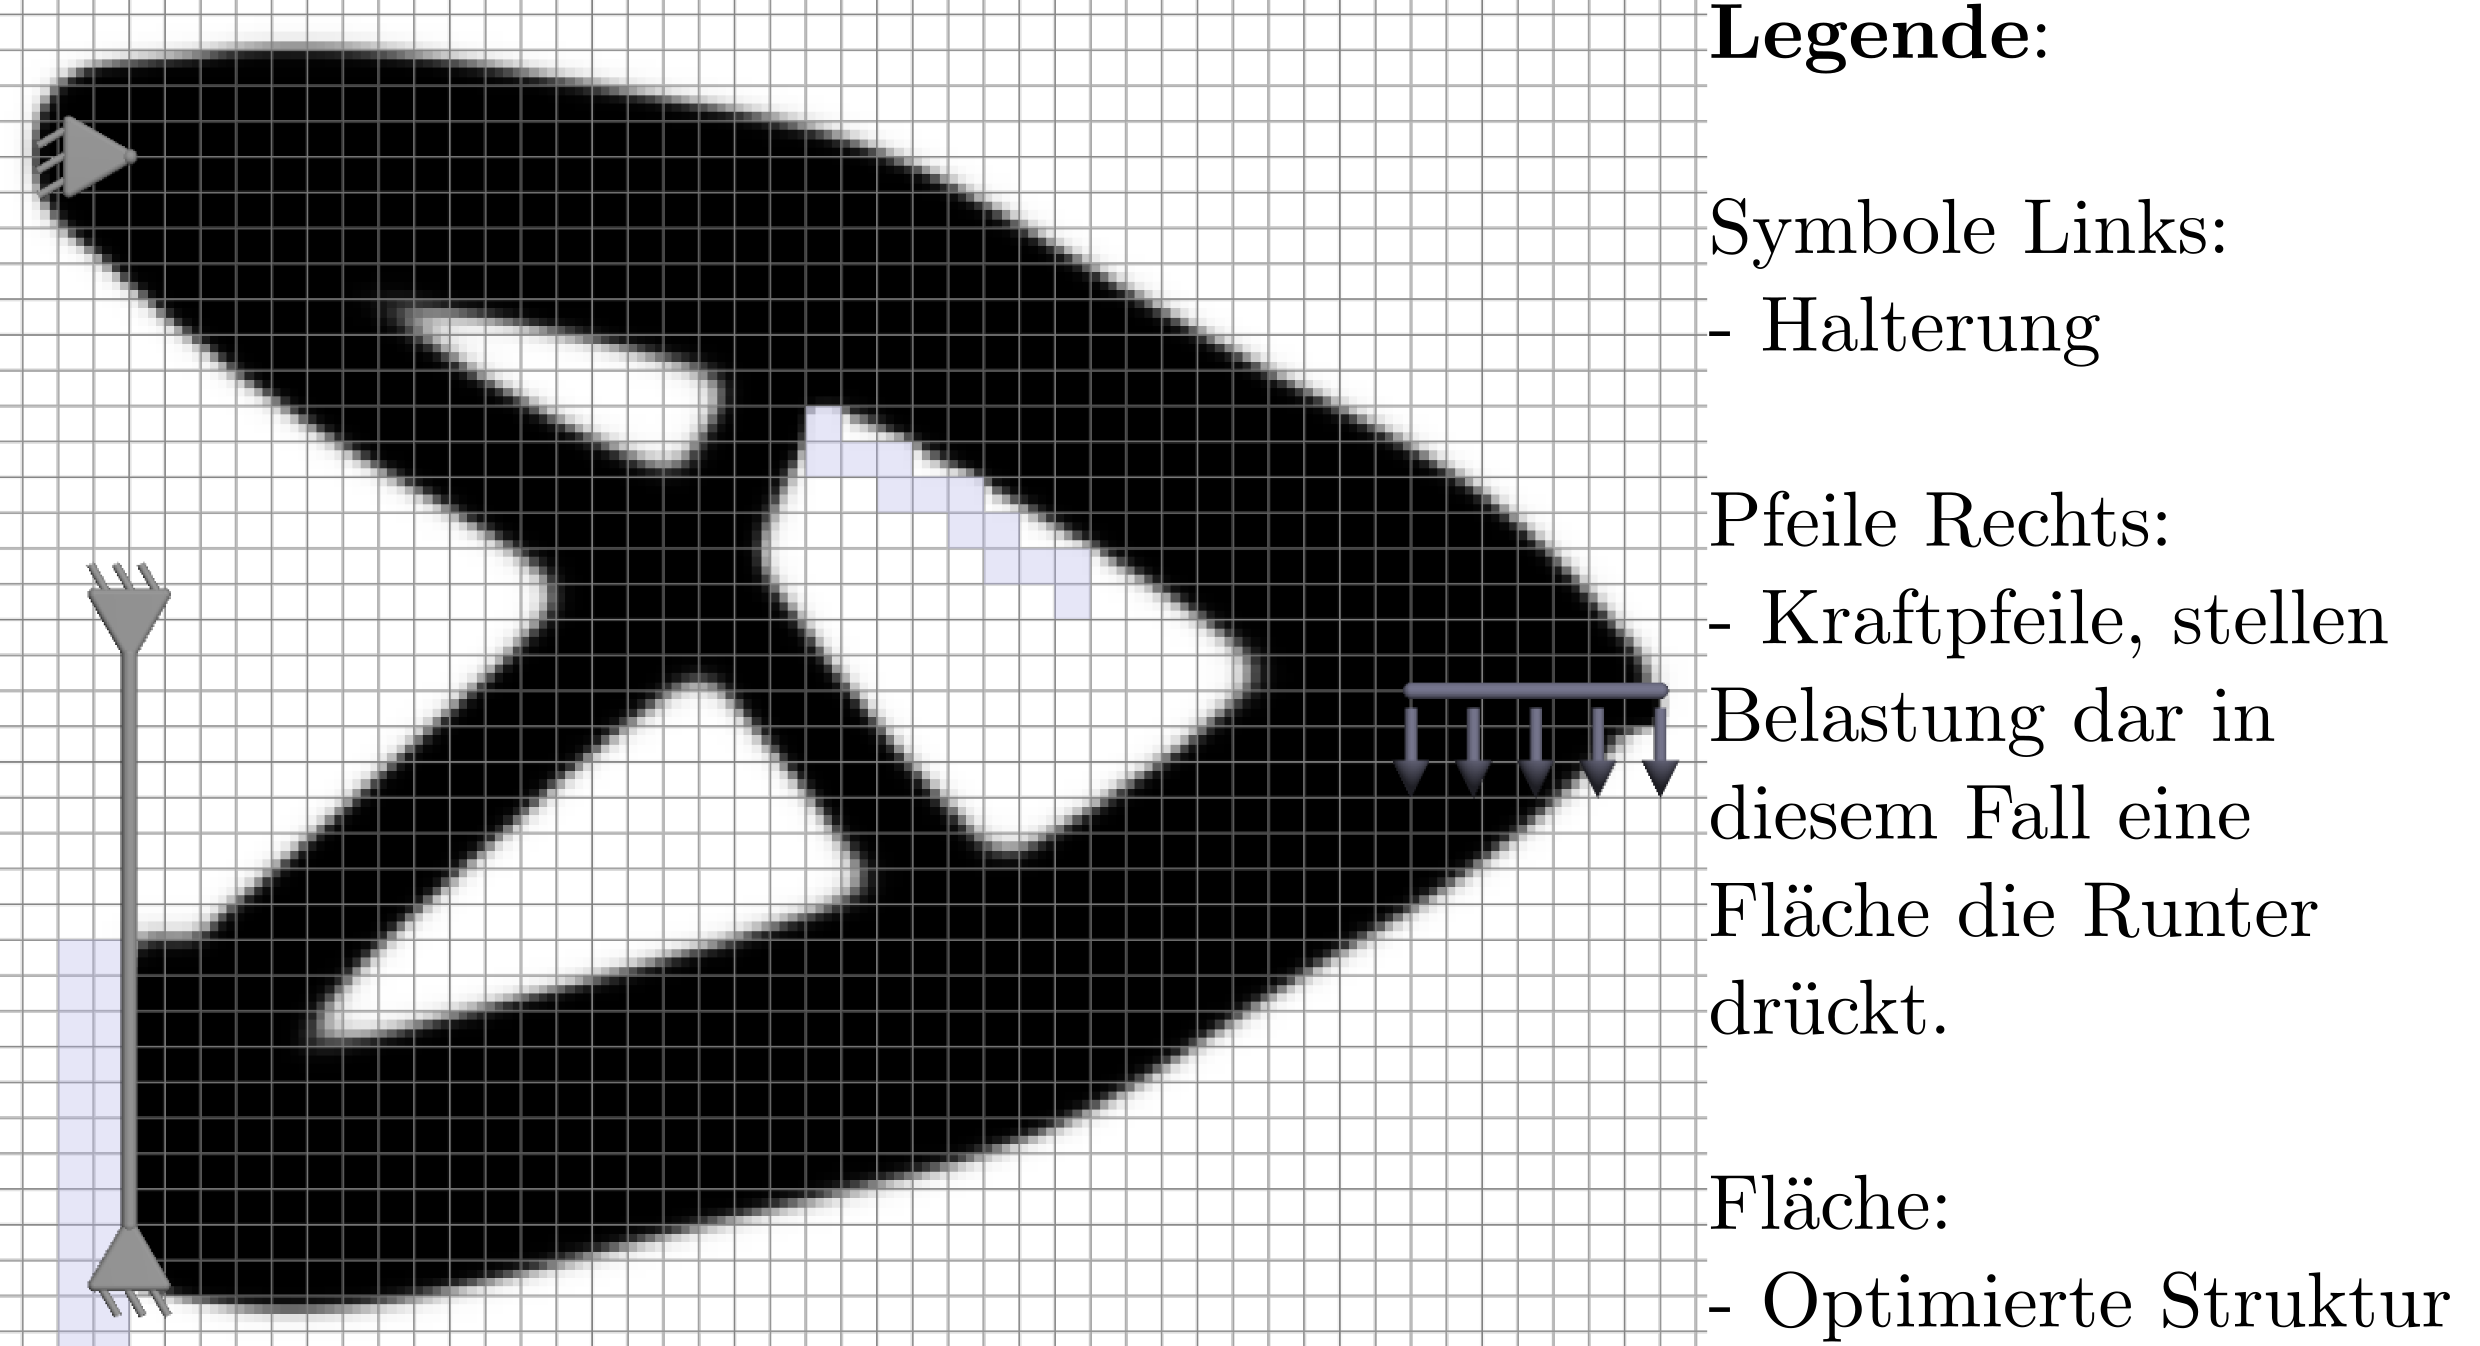
\includegraphics[width=1\textwidth]{figures/legende.png}
    \caption{Legende zur Simulation}
    \label{fig:legende}
\end{figure}
\end{frame}


\begin{frame}{Topologie Simulieren 3}
\begin{figure}[H]
    \begin{minipage}{0.25\textwidth}
        \centering
        \includegraphics[width=\linewidth]{figures/brücke.png}
        \caption{Br\"ucke}
        \label{fig:bruecke}
    \end{minipage}\hfill
    \begin{minipage}{0.25\textwidth}
        \centering
        \includegraphics[width=\linewidth]{figures/Fläche.png}
        \caption{Tragfl\"ache}
    \end{minipage}\hfill
    \begin{minipage}{0.25\textwidth}
        \centering
        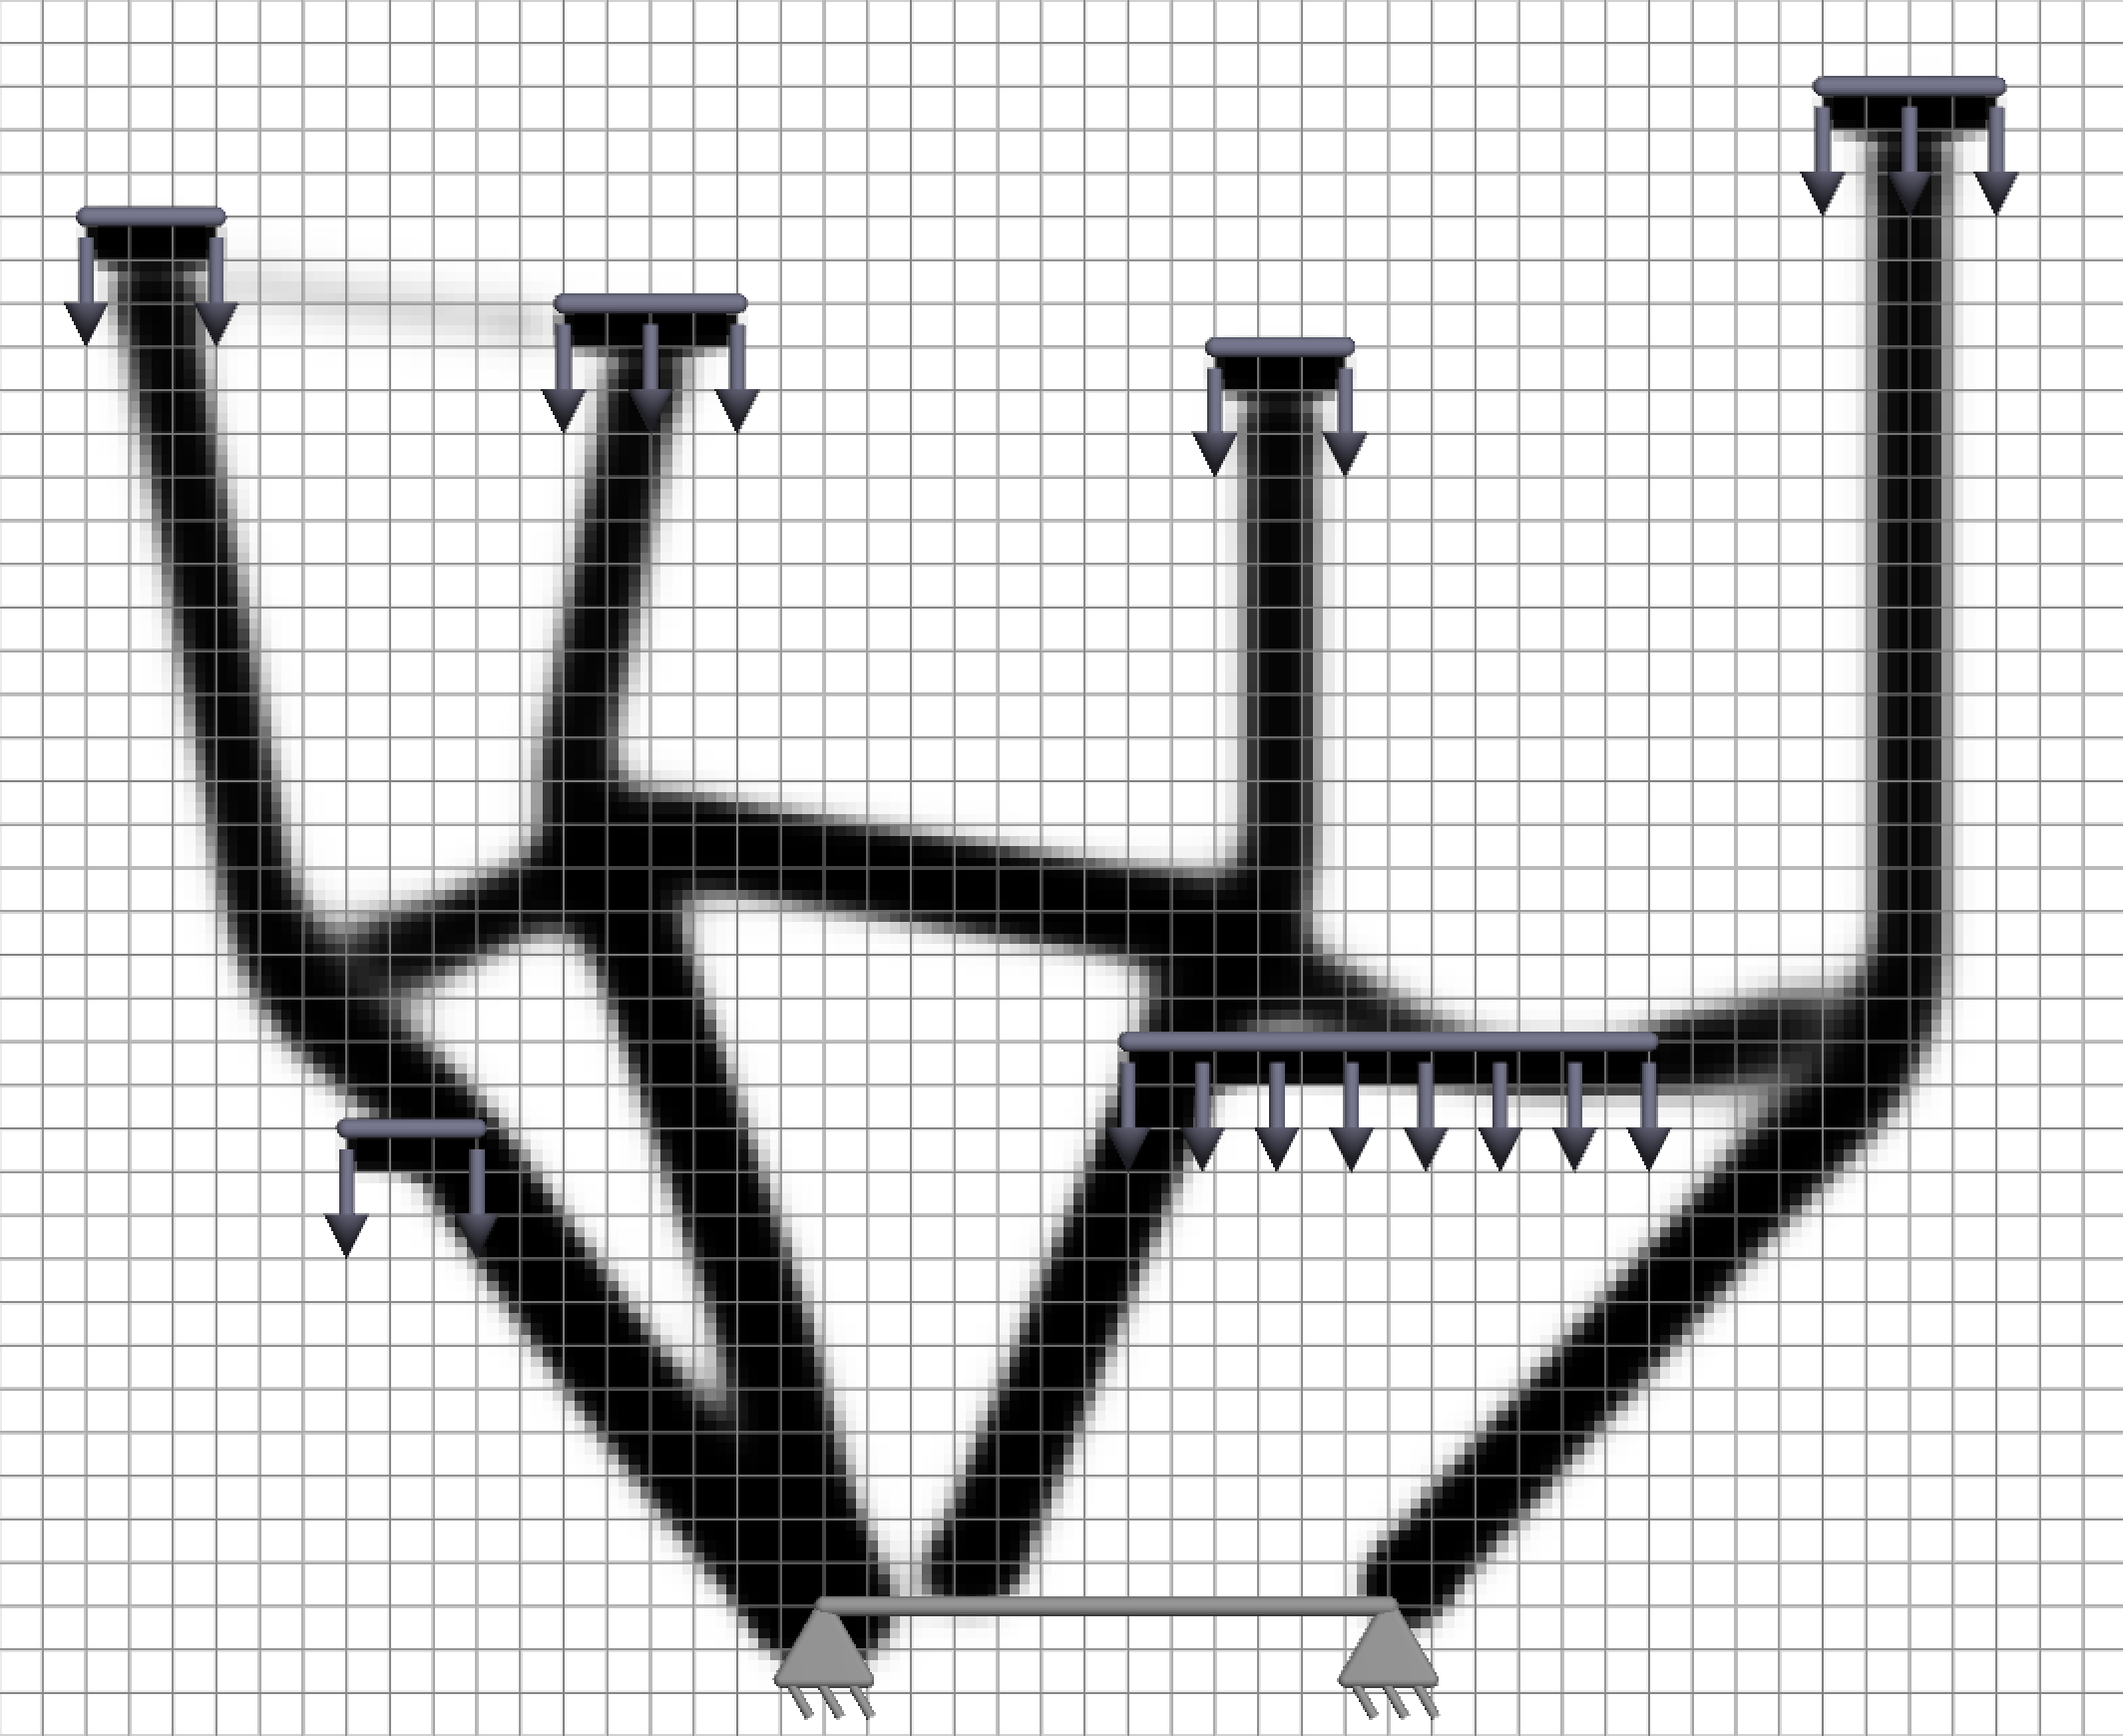
\includegraphics[width=\linewidth]{figures/baum.png}
        \caption{Baum}
    \end{minipage}
\end{figure}

\end{frame}


\begin{frame}{Topologie Simulieren 4}
\begin{figure}[H]
    \begin{minipage}{0.25\textwidth}
        \centering
        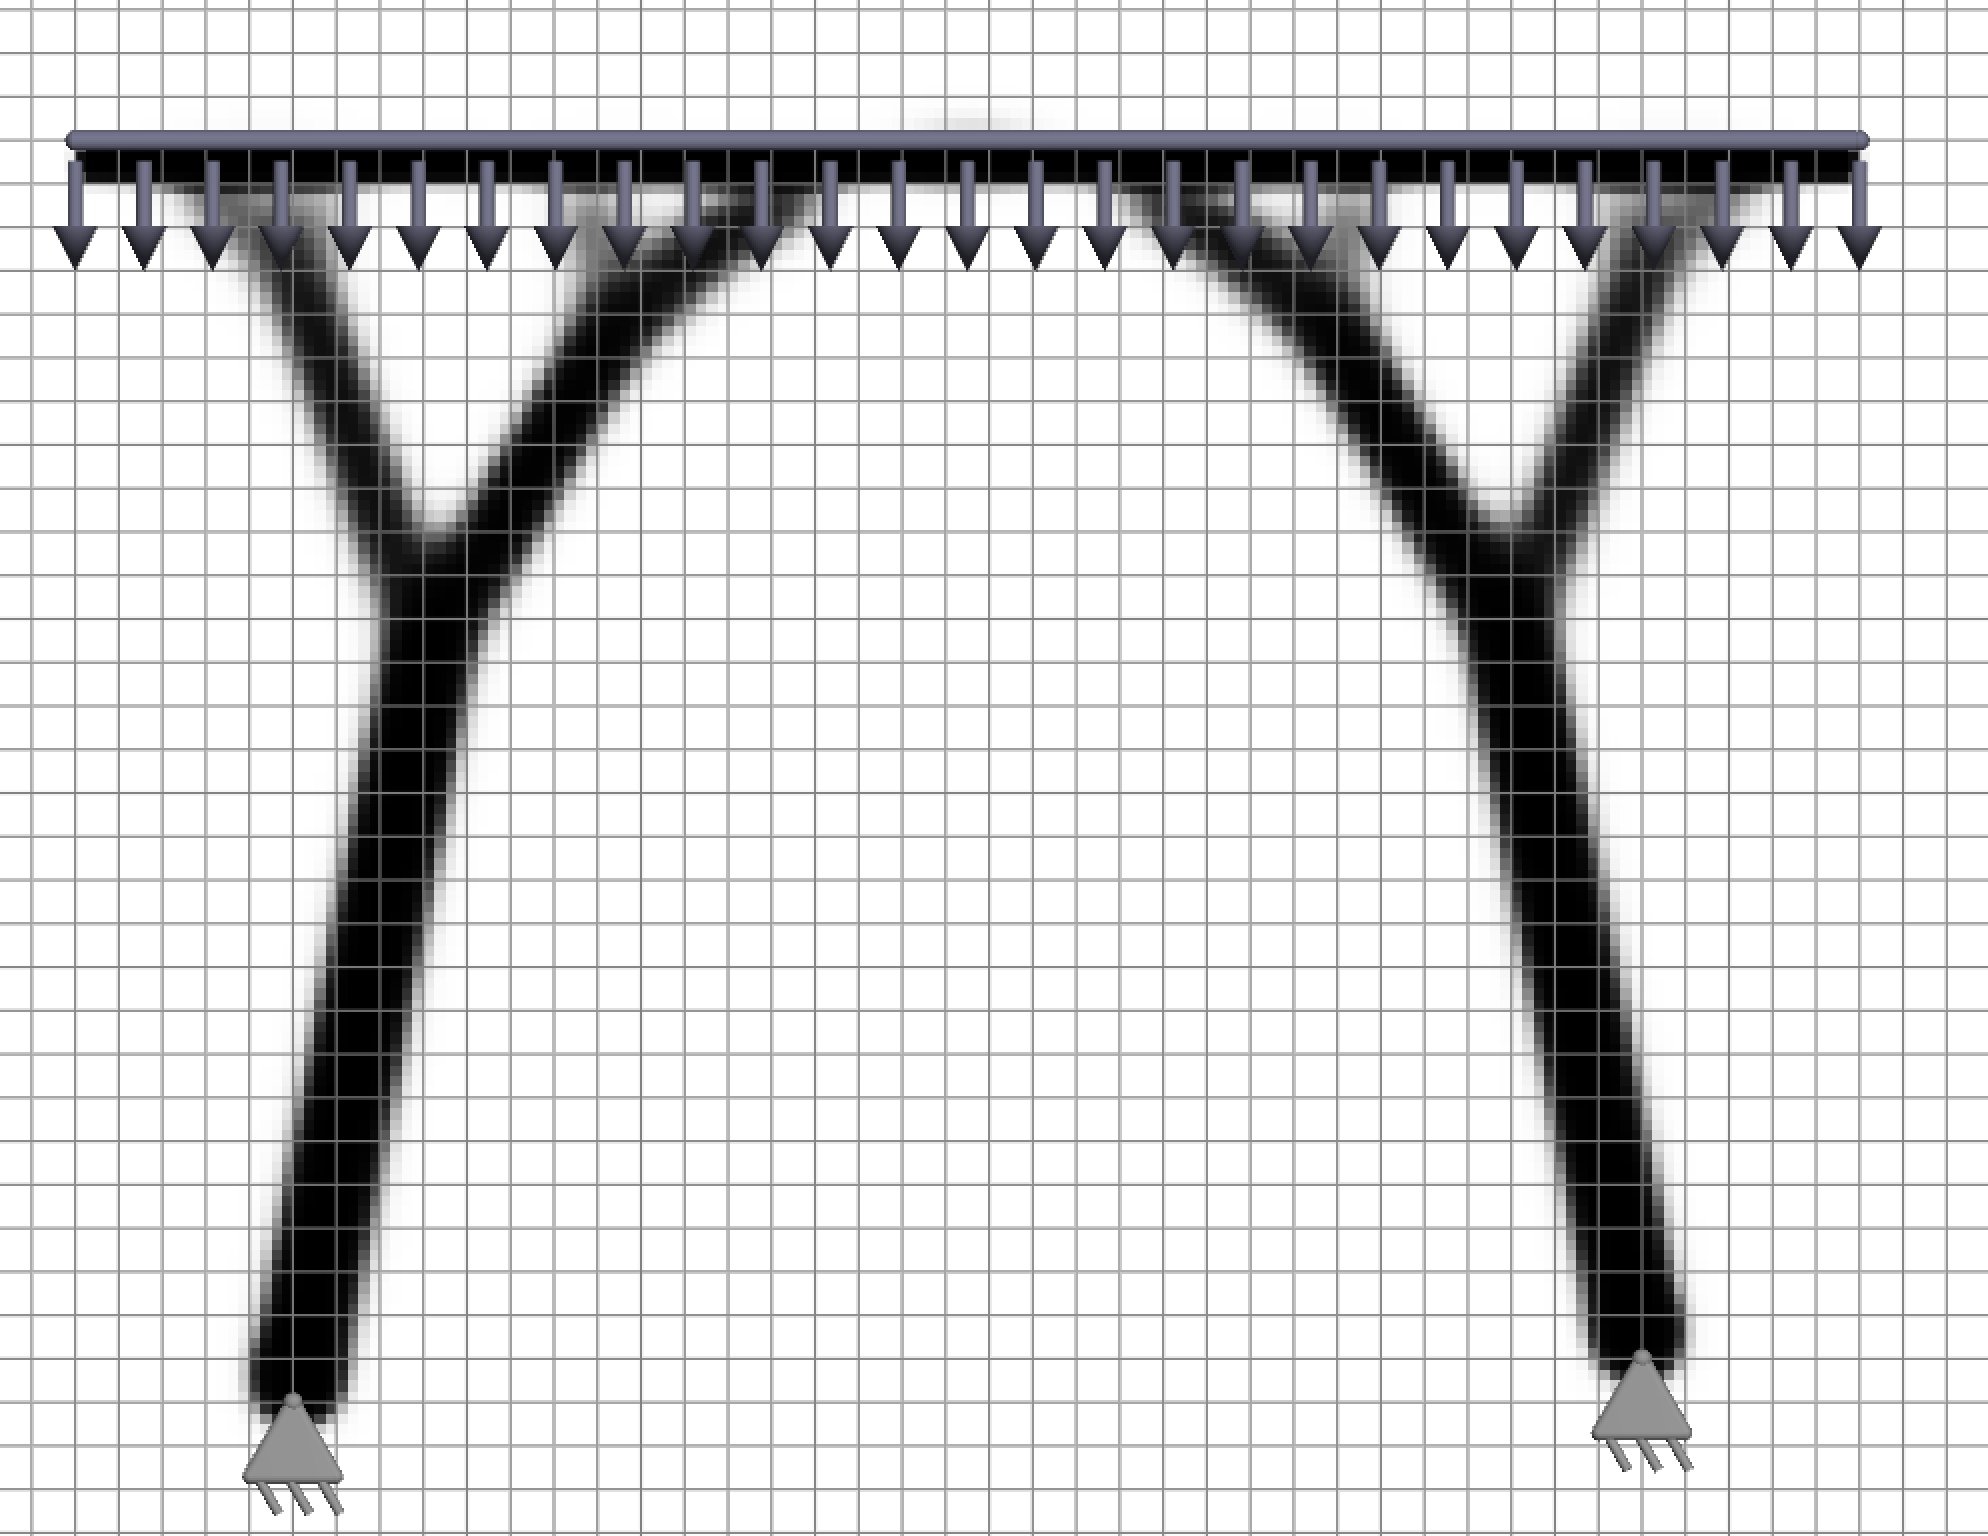
\includegraphics[width=\linewidth]{figures/tisch.png}
        \caption{Tisch}
    \end{minipage}\hfill
    \begin{minipage}{0.25\textwidth}
        \centering
        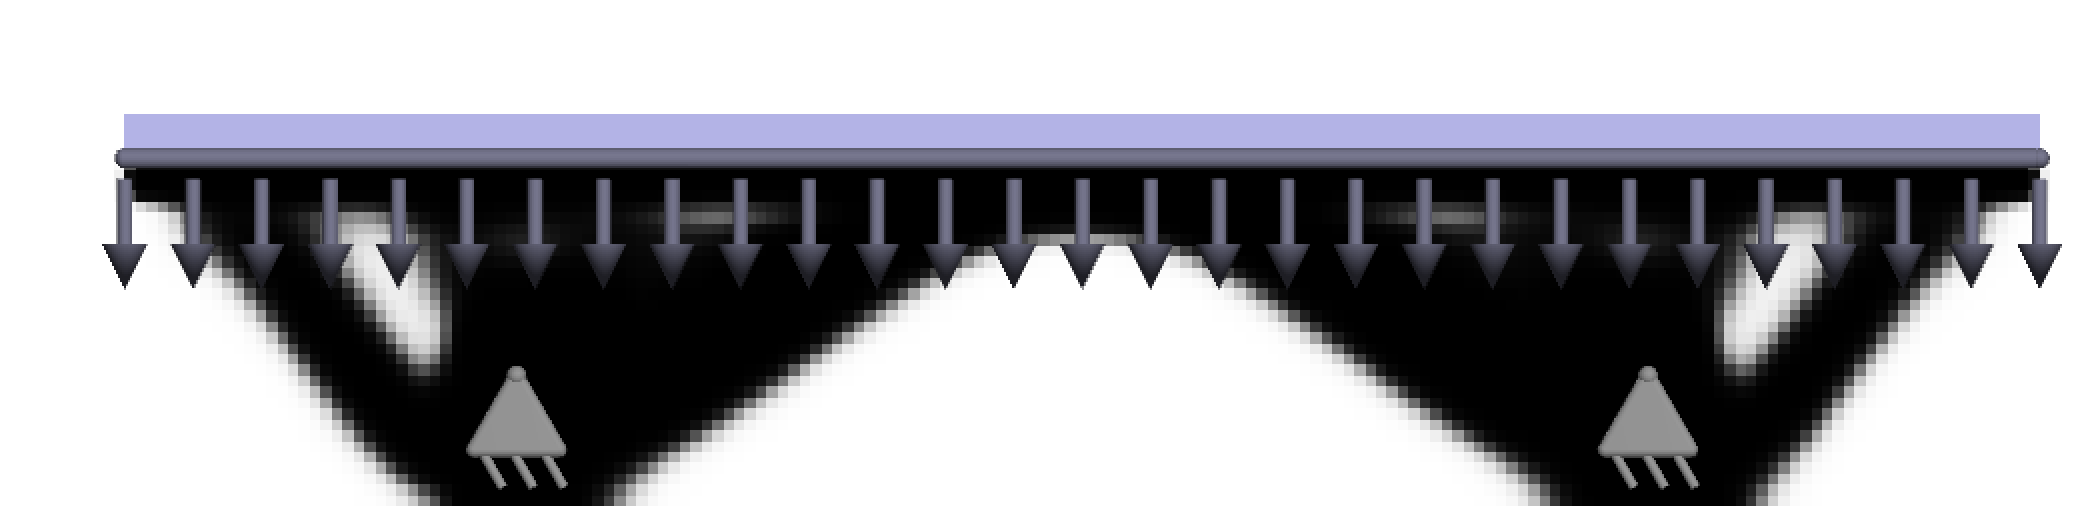
\includegraphics[width=\linewidth]{figures/Palette.png}
        \caption{Palette}
    \end{minipage}\hfill
    \begin{minipage}{0.25\textwidth}
        \centering
        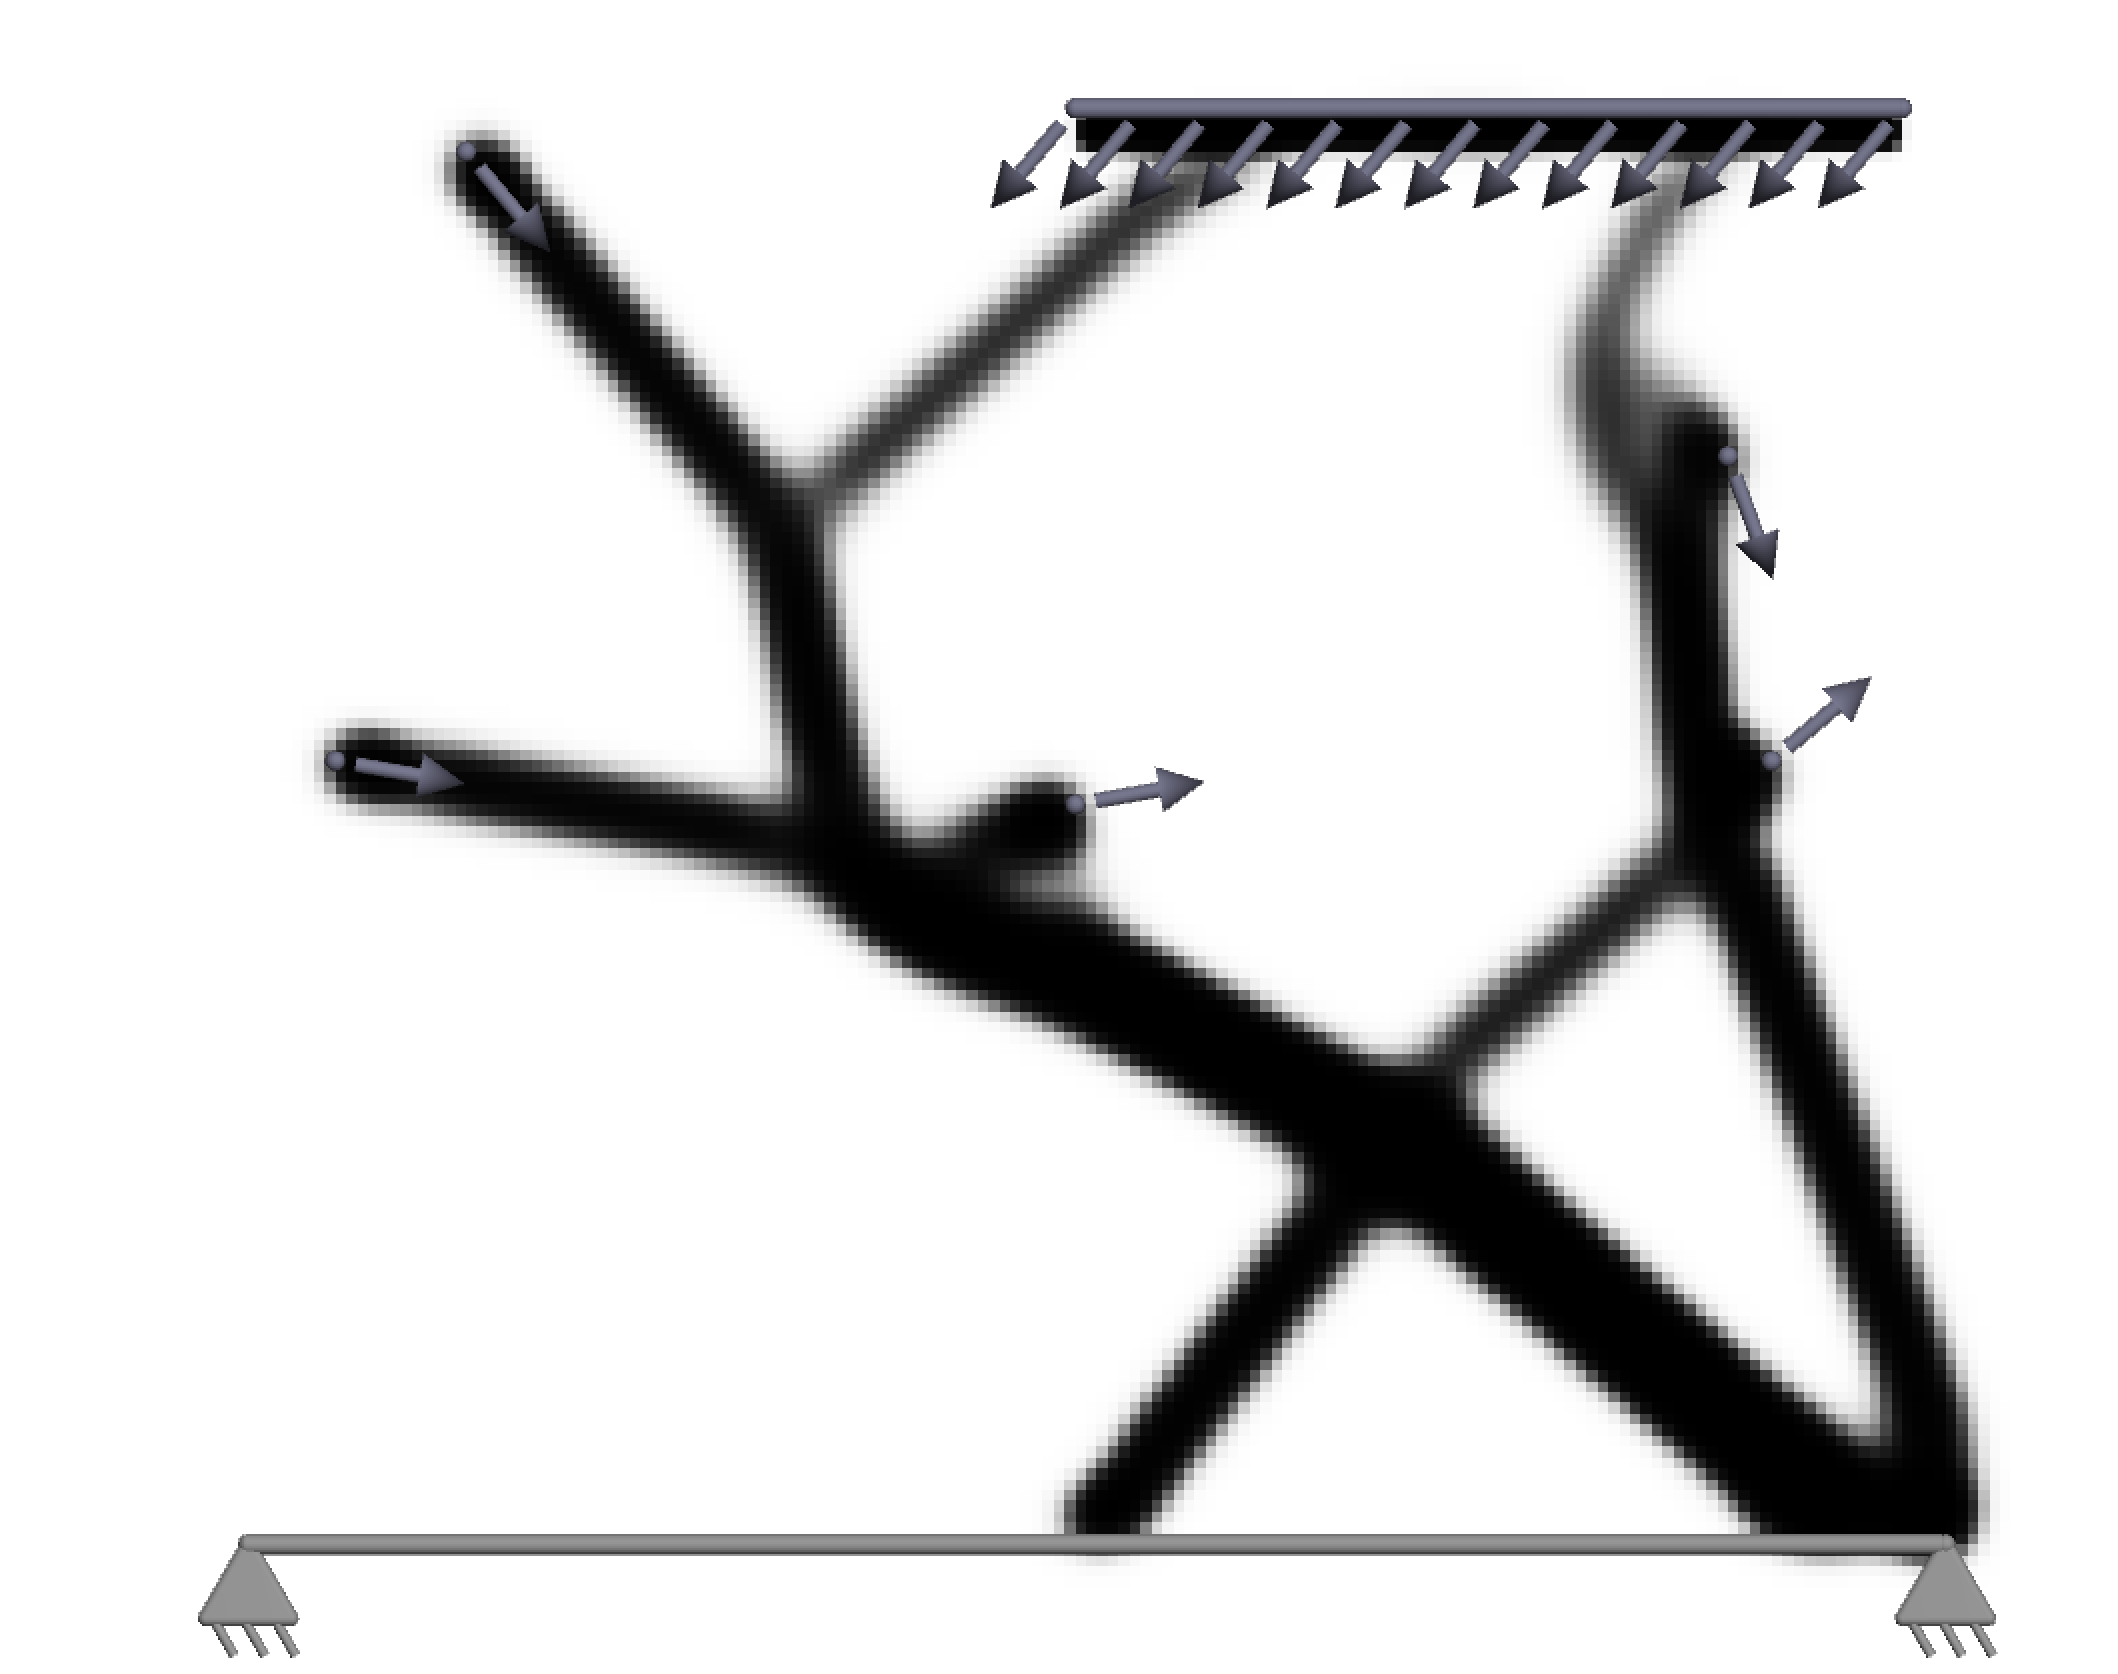
\includegraphics[width=\linewidth]{figures/abstrakt.png}
        \caption{Abstrakteres Gebilde}
    \end{minipage}
\end{figure}
\end{frame}



\begin{frame}{Topologie Simulieren 5}
\begin{figure}[H]
    \begin{minipage}{0.4\textwidth}
        \centering
        \includegraphics[width=\linewidth]{figures/brücke.png}
        \caption{Simulierte Br\"ucke}
    \end{minipage}\hfill
    \begin{minipage}{0.4\textwidth}
        \centering
        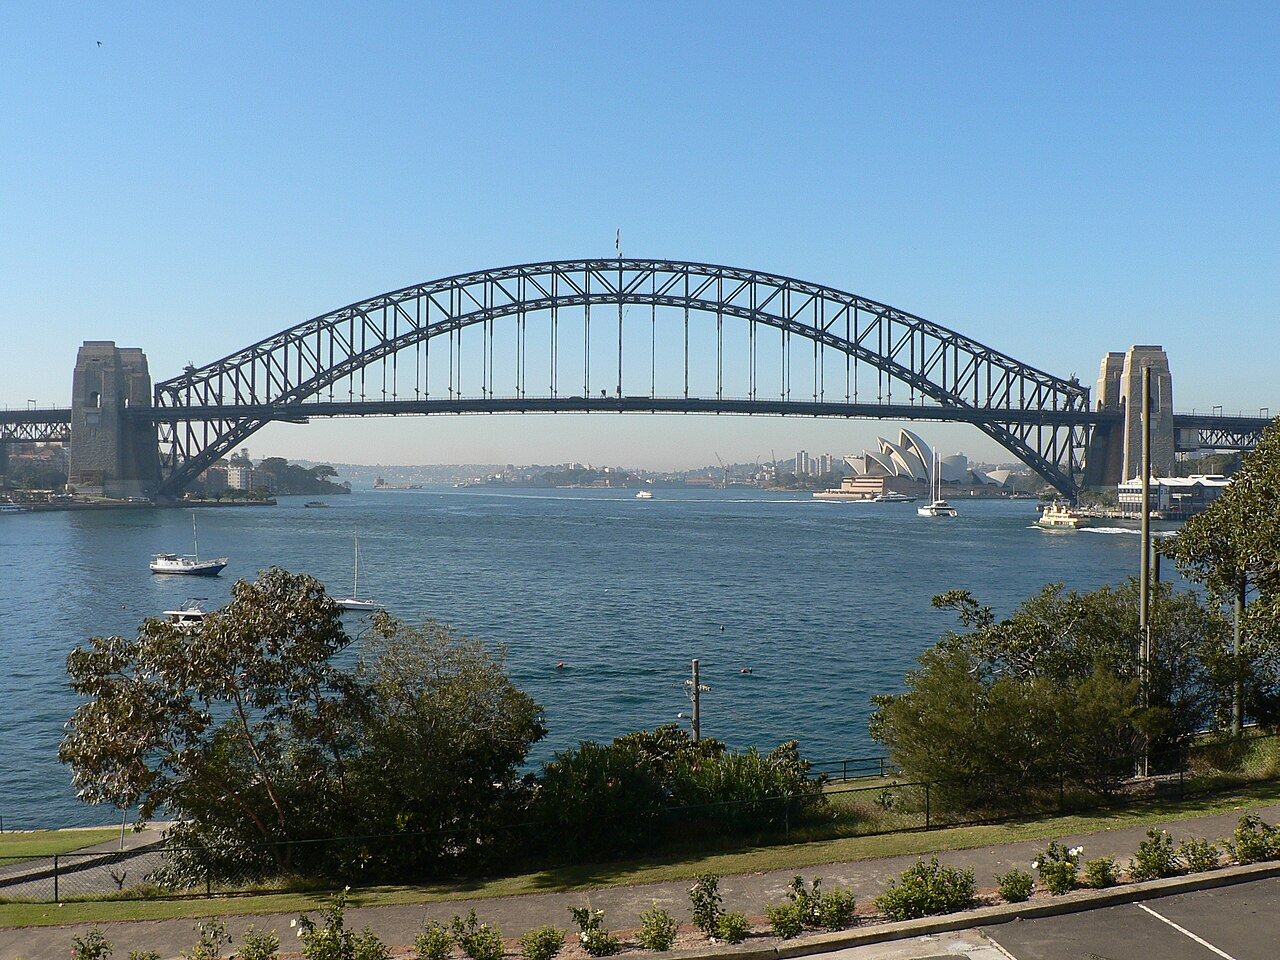
\includegraphics[width=\linewidth]{figures/Sydney-Harbour_bridge.JPG}
        \caption{Hafen Br\"ucke Sydney\parencite{rabich2023}}
    \end{minipage}
\end{figure}
\end{frame}



\section{FDM-Druck}
\begin{frame}{Verfahren und Baustoffe}

\subsubsection{Beton}
    \begin{figure}[H]
        \centering
        \begin{minipage}{0.3\textwidth}
           \centering
           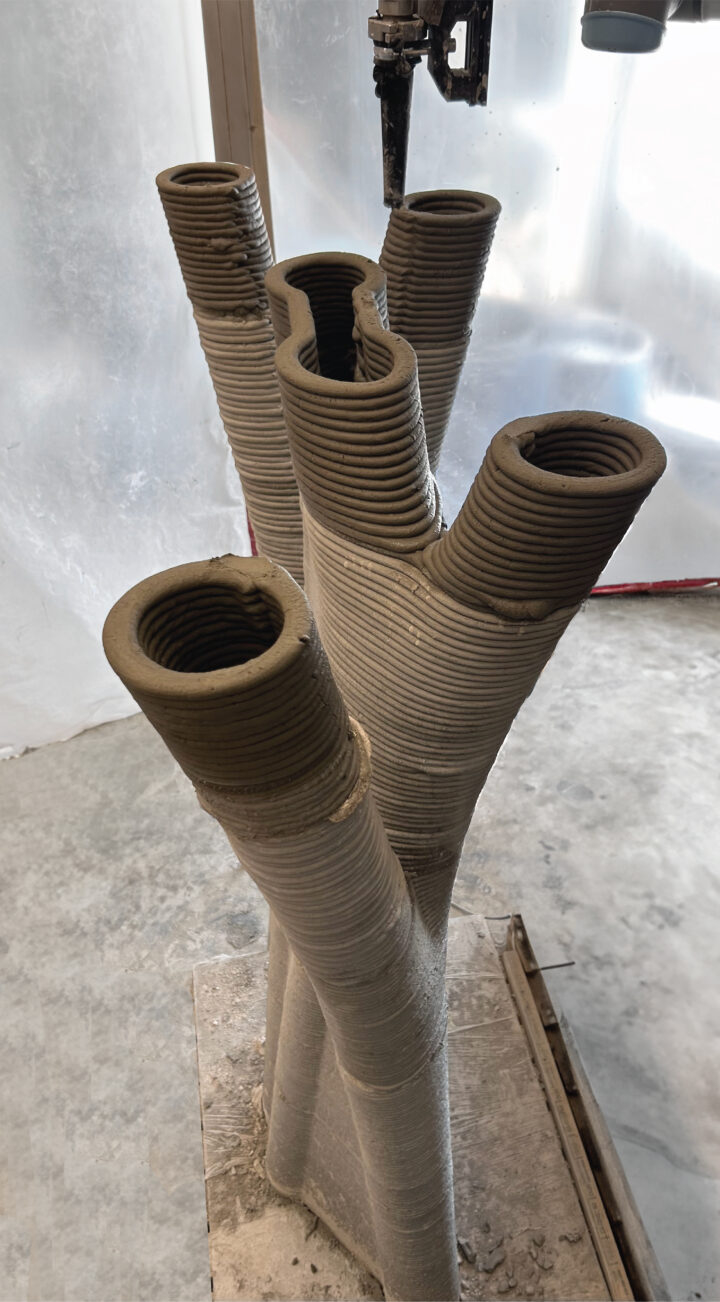
\includegraphics[width=\linewidth]{figures/beispiele/meibodi-2023-1.jpg}
           \caption{Gedruckte Betonstrucktur leer \parencite{meibodi2023}}
           \label{fig:leer}
        \end{minipage}
        \begin{minipage}{0.3\textwidth}
           \centering
           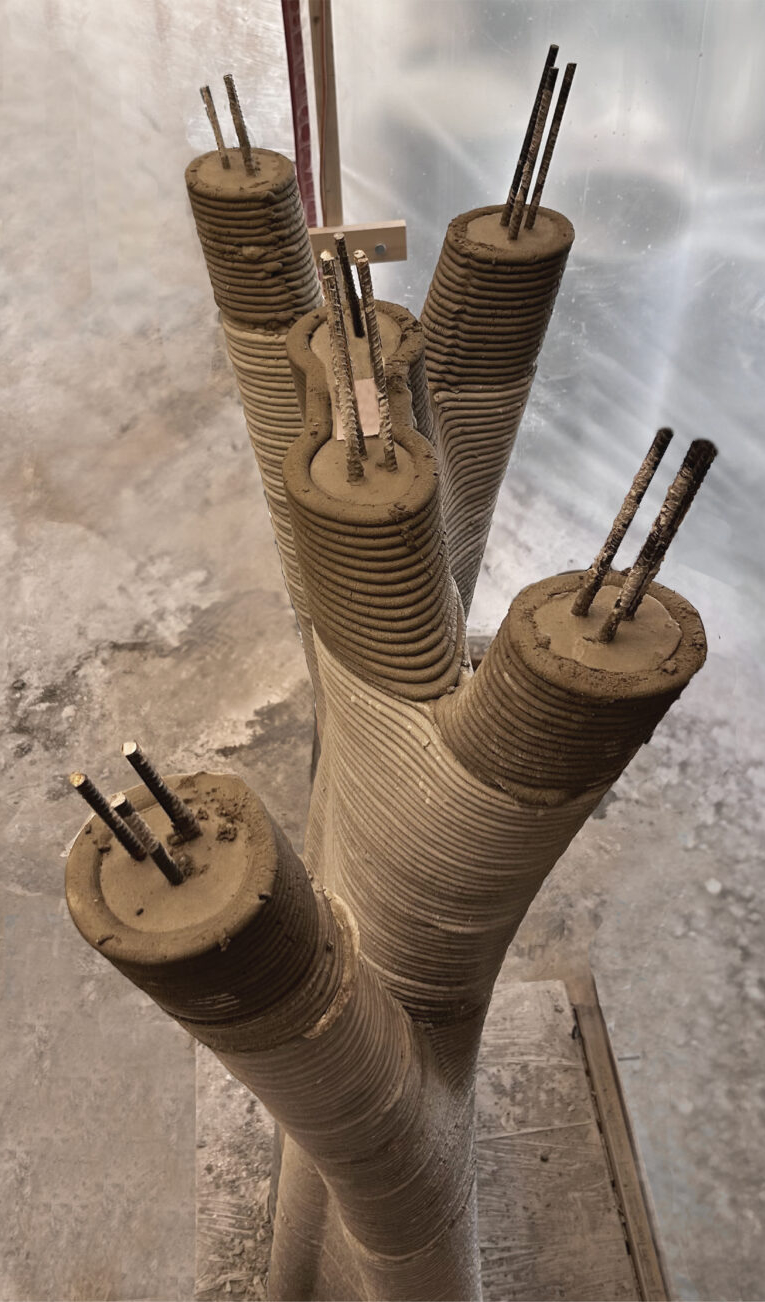
\includegraphics[width=\linewidth]{figures/beispiele/meibodi-2023-2.jpg}
           \caption{Gedruckte Betonstrucktur gef\"ullt \parencite{meibodi2023}}
           \label{fig:voll}
        \end{minipage}
        \begin{minipage}{0.3\textwidth}
            \begin{itemize}
                \item Beispiel vom DART Lab Michigan. 
                \item Gebilde Parametrisch erzeugt
                \item Modell ist Gedruckt, wie rechts am Ende Massivbeton und Stahlverst\"arkt
            \end{itemize}
        \end{minipage}
    \end{figure}
\end{frame}

\begin{frame}{Beton 2}
   \begin{figure}[htpb]
       \centering
       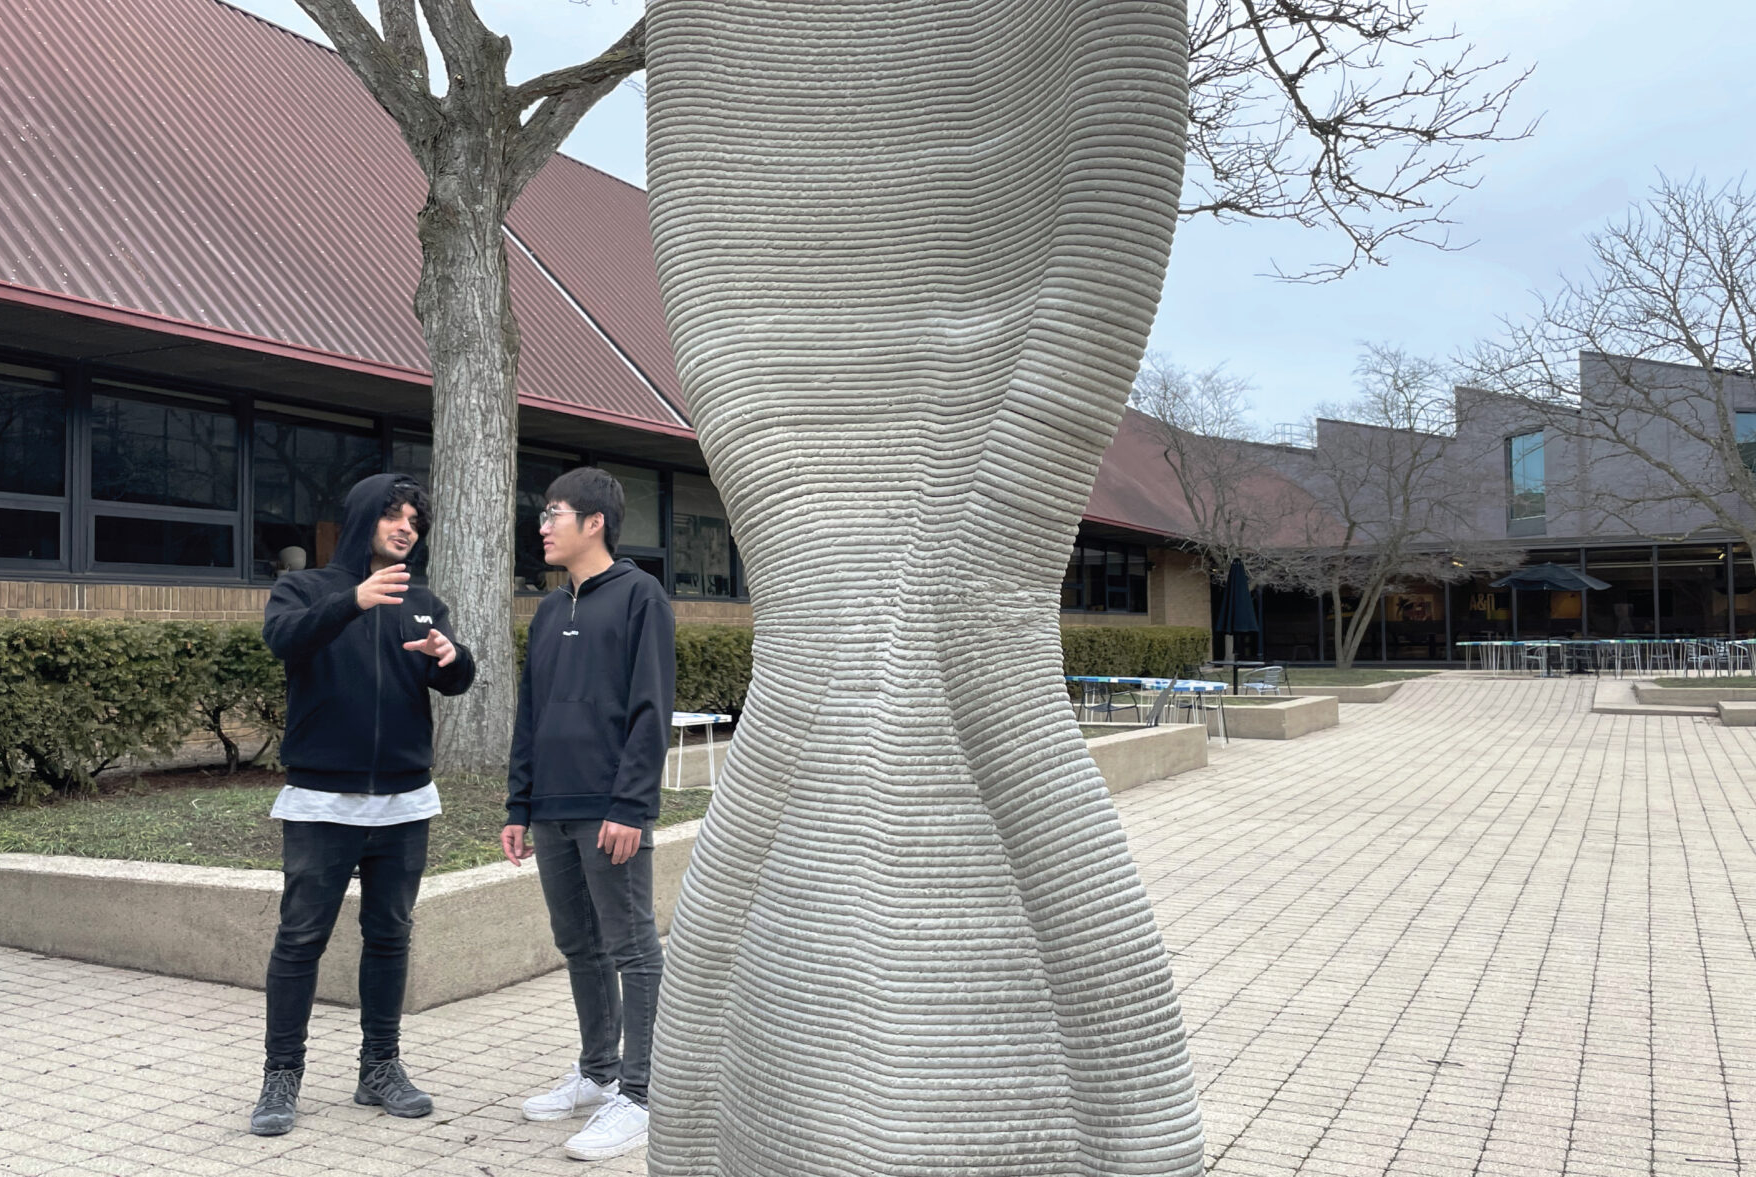
\includegraphics[width=0.9\textwidth]{figures/beispiele/meibodi-2023-3.jpg}
       \caption{Endergebnis}
       \label{fig:meibodi-2023-3}
   \end{figure} 
\end{frame}



%\begin{frame}{3d-Druck in der Architektur}
%
%\end{frame}

\begin{frame}{Problem}
    \begin{itemize}
        \item Viel Baumaterial das nicht nachhaltig ist muss weggeworfen werden.
        \item Muss aber jedes mal Passgenau konstruiert werden.
        \item $\implies$ teuer \& und un\"otig
    \end{itemize}
    \begin{figure}[H]
        \begin{minipage}{0.4\textwidth}
           \centering
           \vfill
           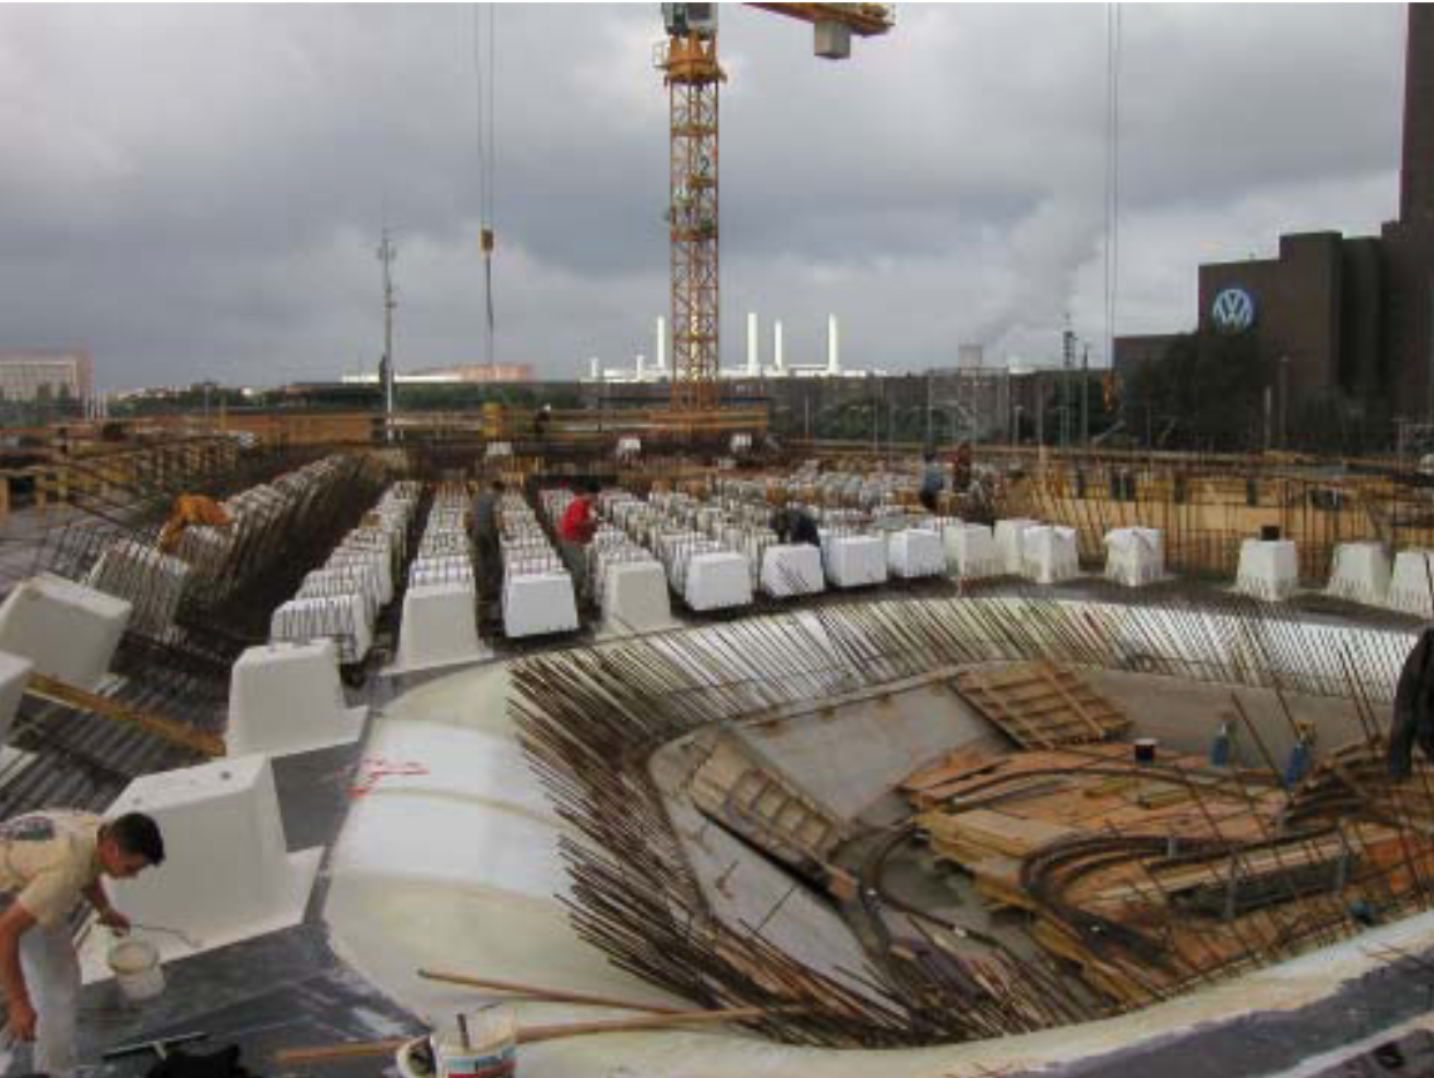
\includegraphics[width=\linewidth]{figures/beispiele/phaeno-307-1.png}
           \caption{Ph\ae{}no Bau \parencite{mayer}}
           \label{fig:bau-phae-1}
        \end{minipage}
            \hfill
        \begin{minipage}{0.4\textwidth}
           \centering
           \vfill
           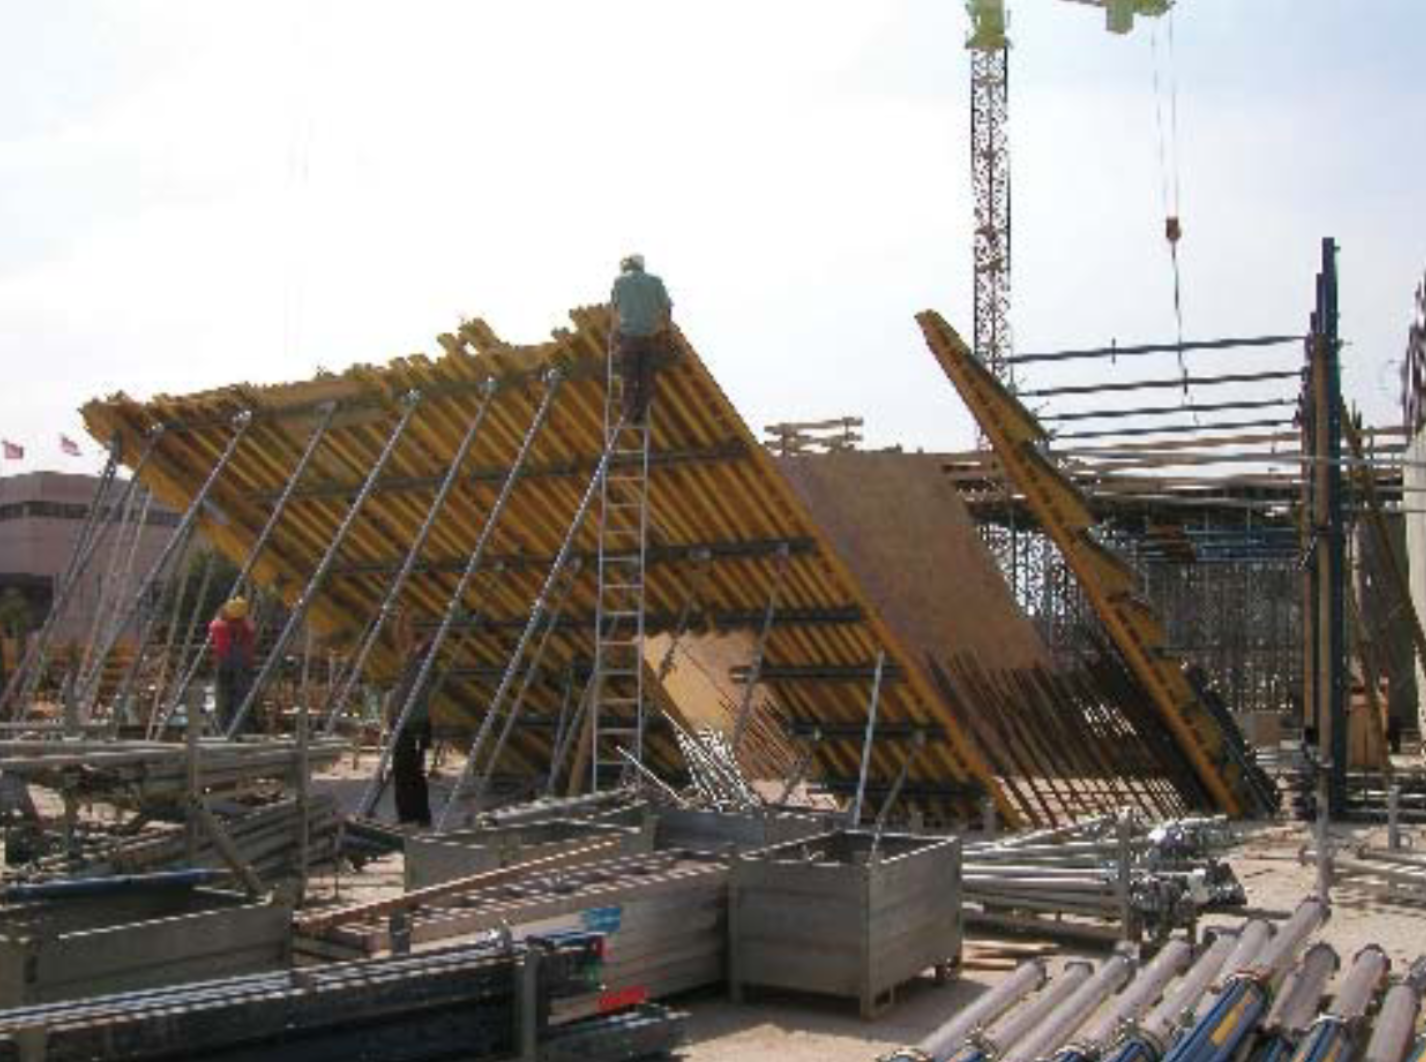
\includegraphics[width=\linewidth]{figures/beispiele/phaeno-307-2.png}
           \caption{Ph\ae{}no Bau \parencite{mayer}}
           \label{fig:bau-phae-2}
        \end{minipage}
    \end{figure}
\end{frame}


\begin{frame}{Pflanzenfasern}
    \begin{figure}[H]
        \begin{minipage}{0.45\textwidth}
           \centering
           \vfill
           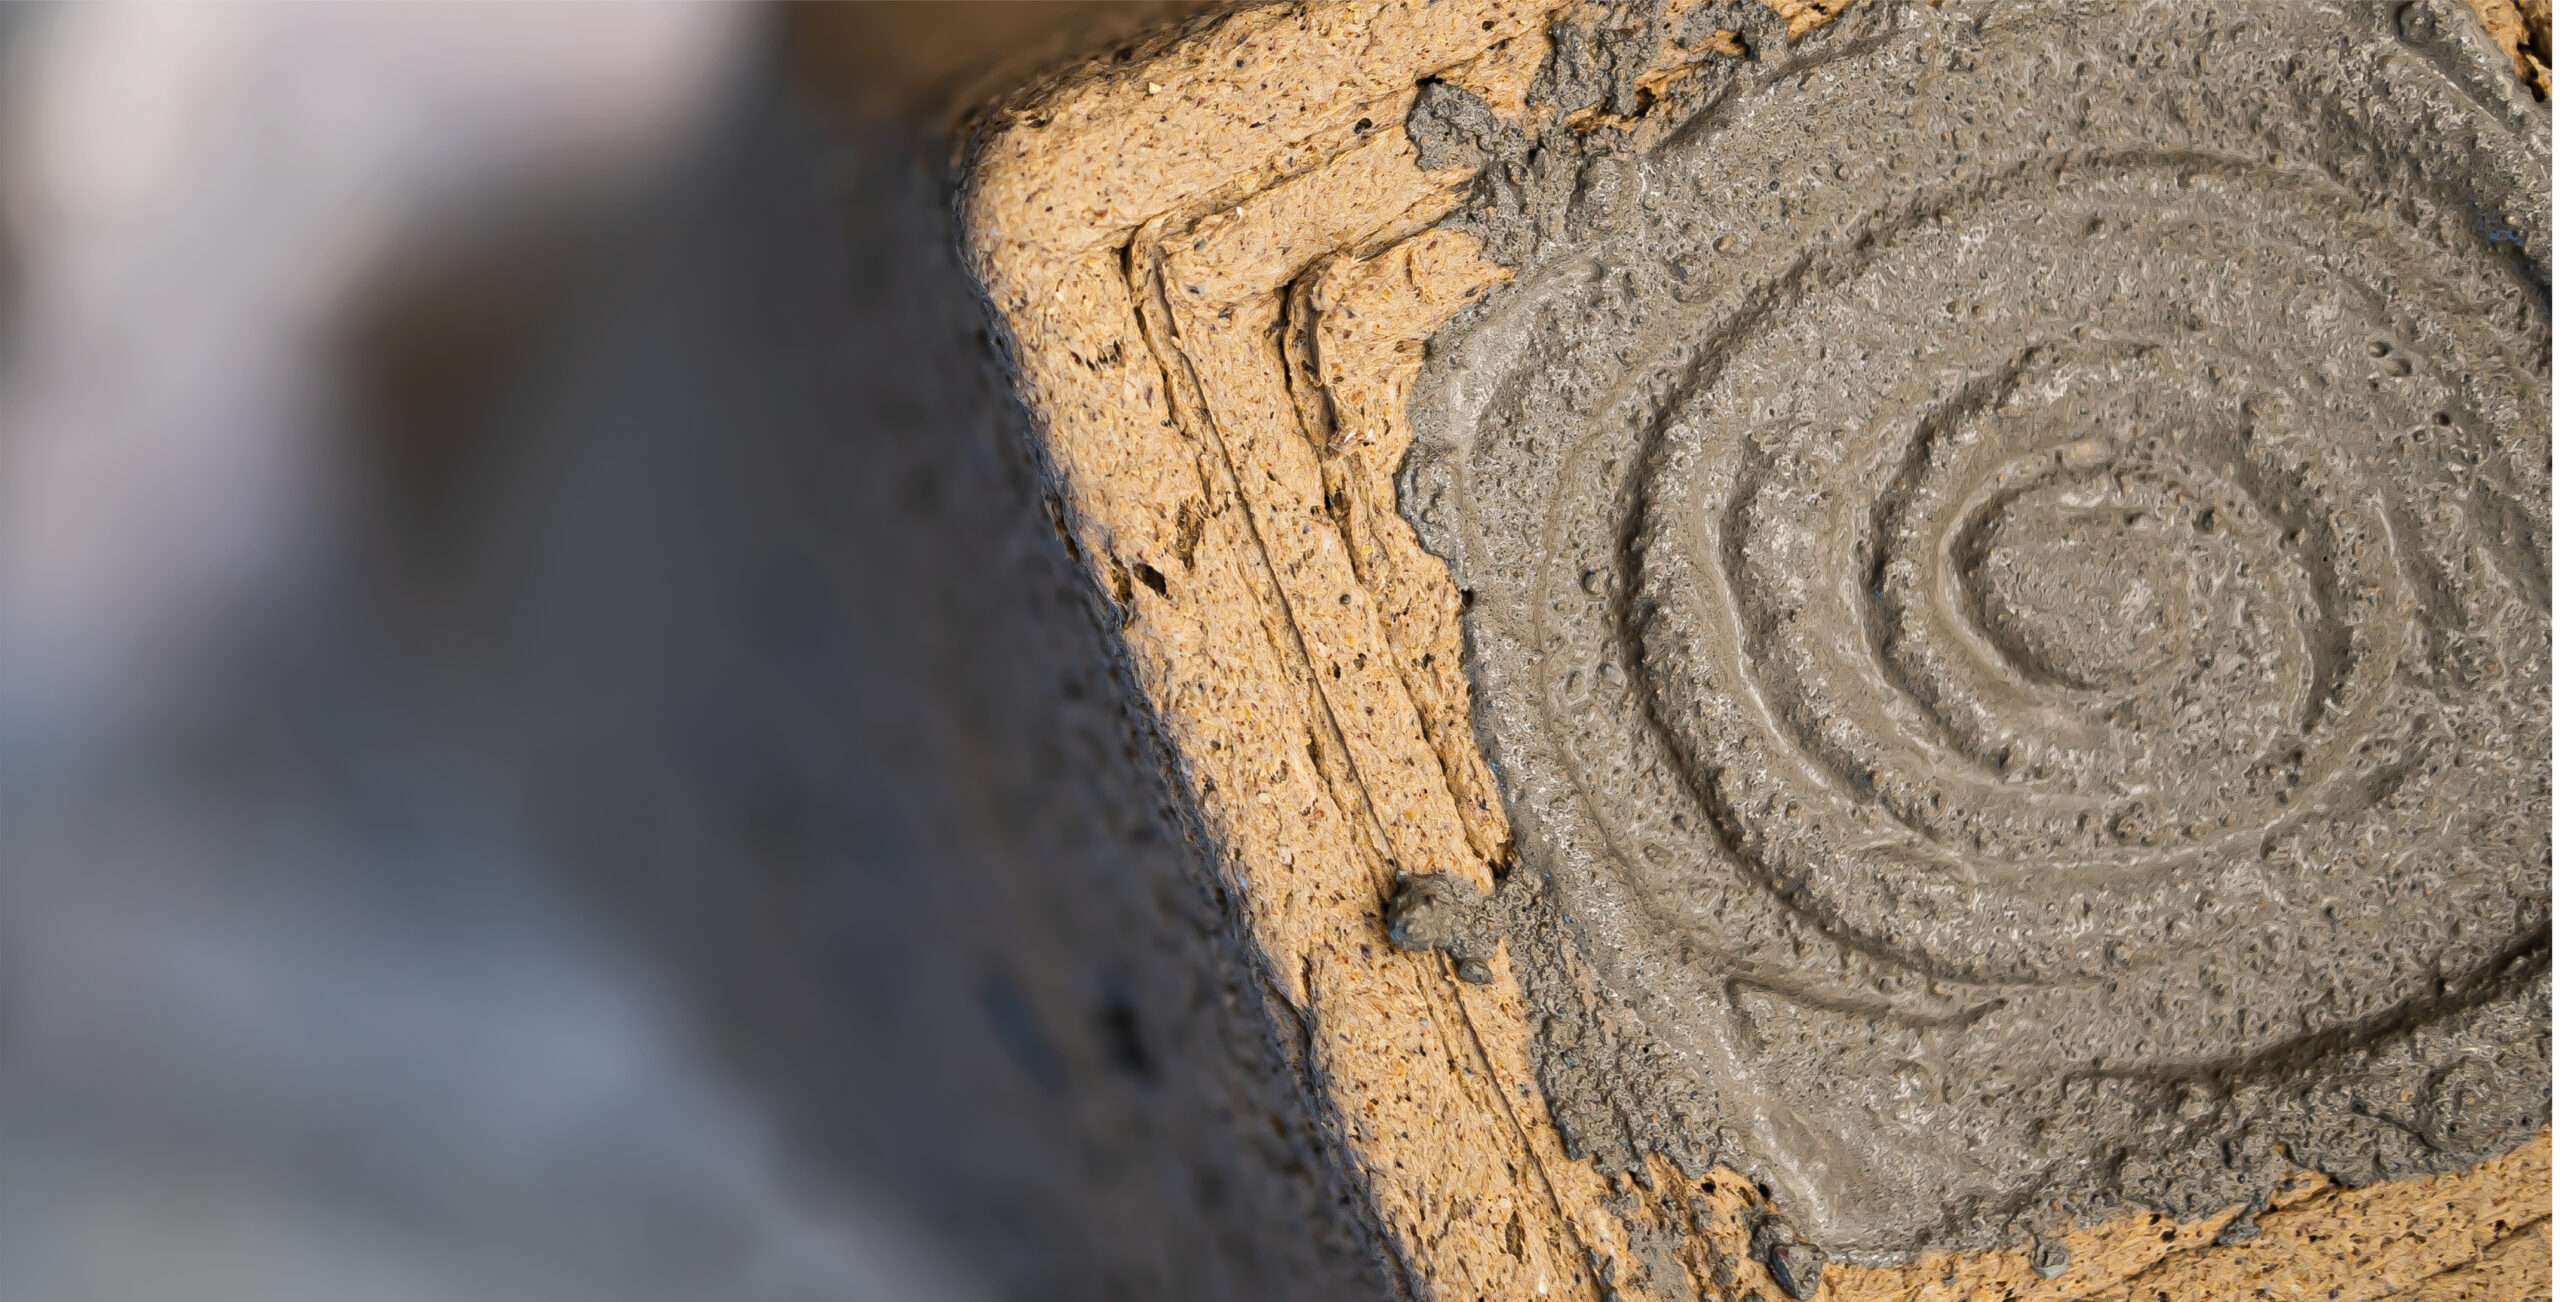
\includegraphics[width=\linewidth]{figures/beispiele/kahn-2023-1.jpg}
           \caption{\parencite{kahn2023}}
           \label{fig:kahn-1}
        \end{minipage}
            \hfill
        \begin{minipage}{0.45\textwidth}
           \centering
           \vfill
           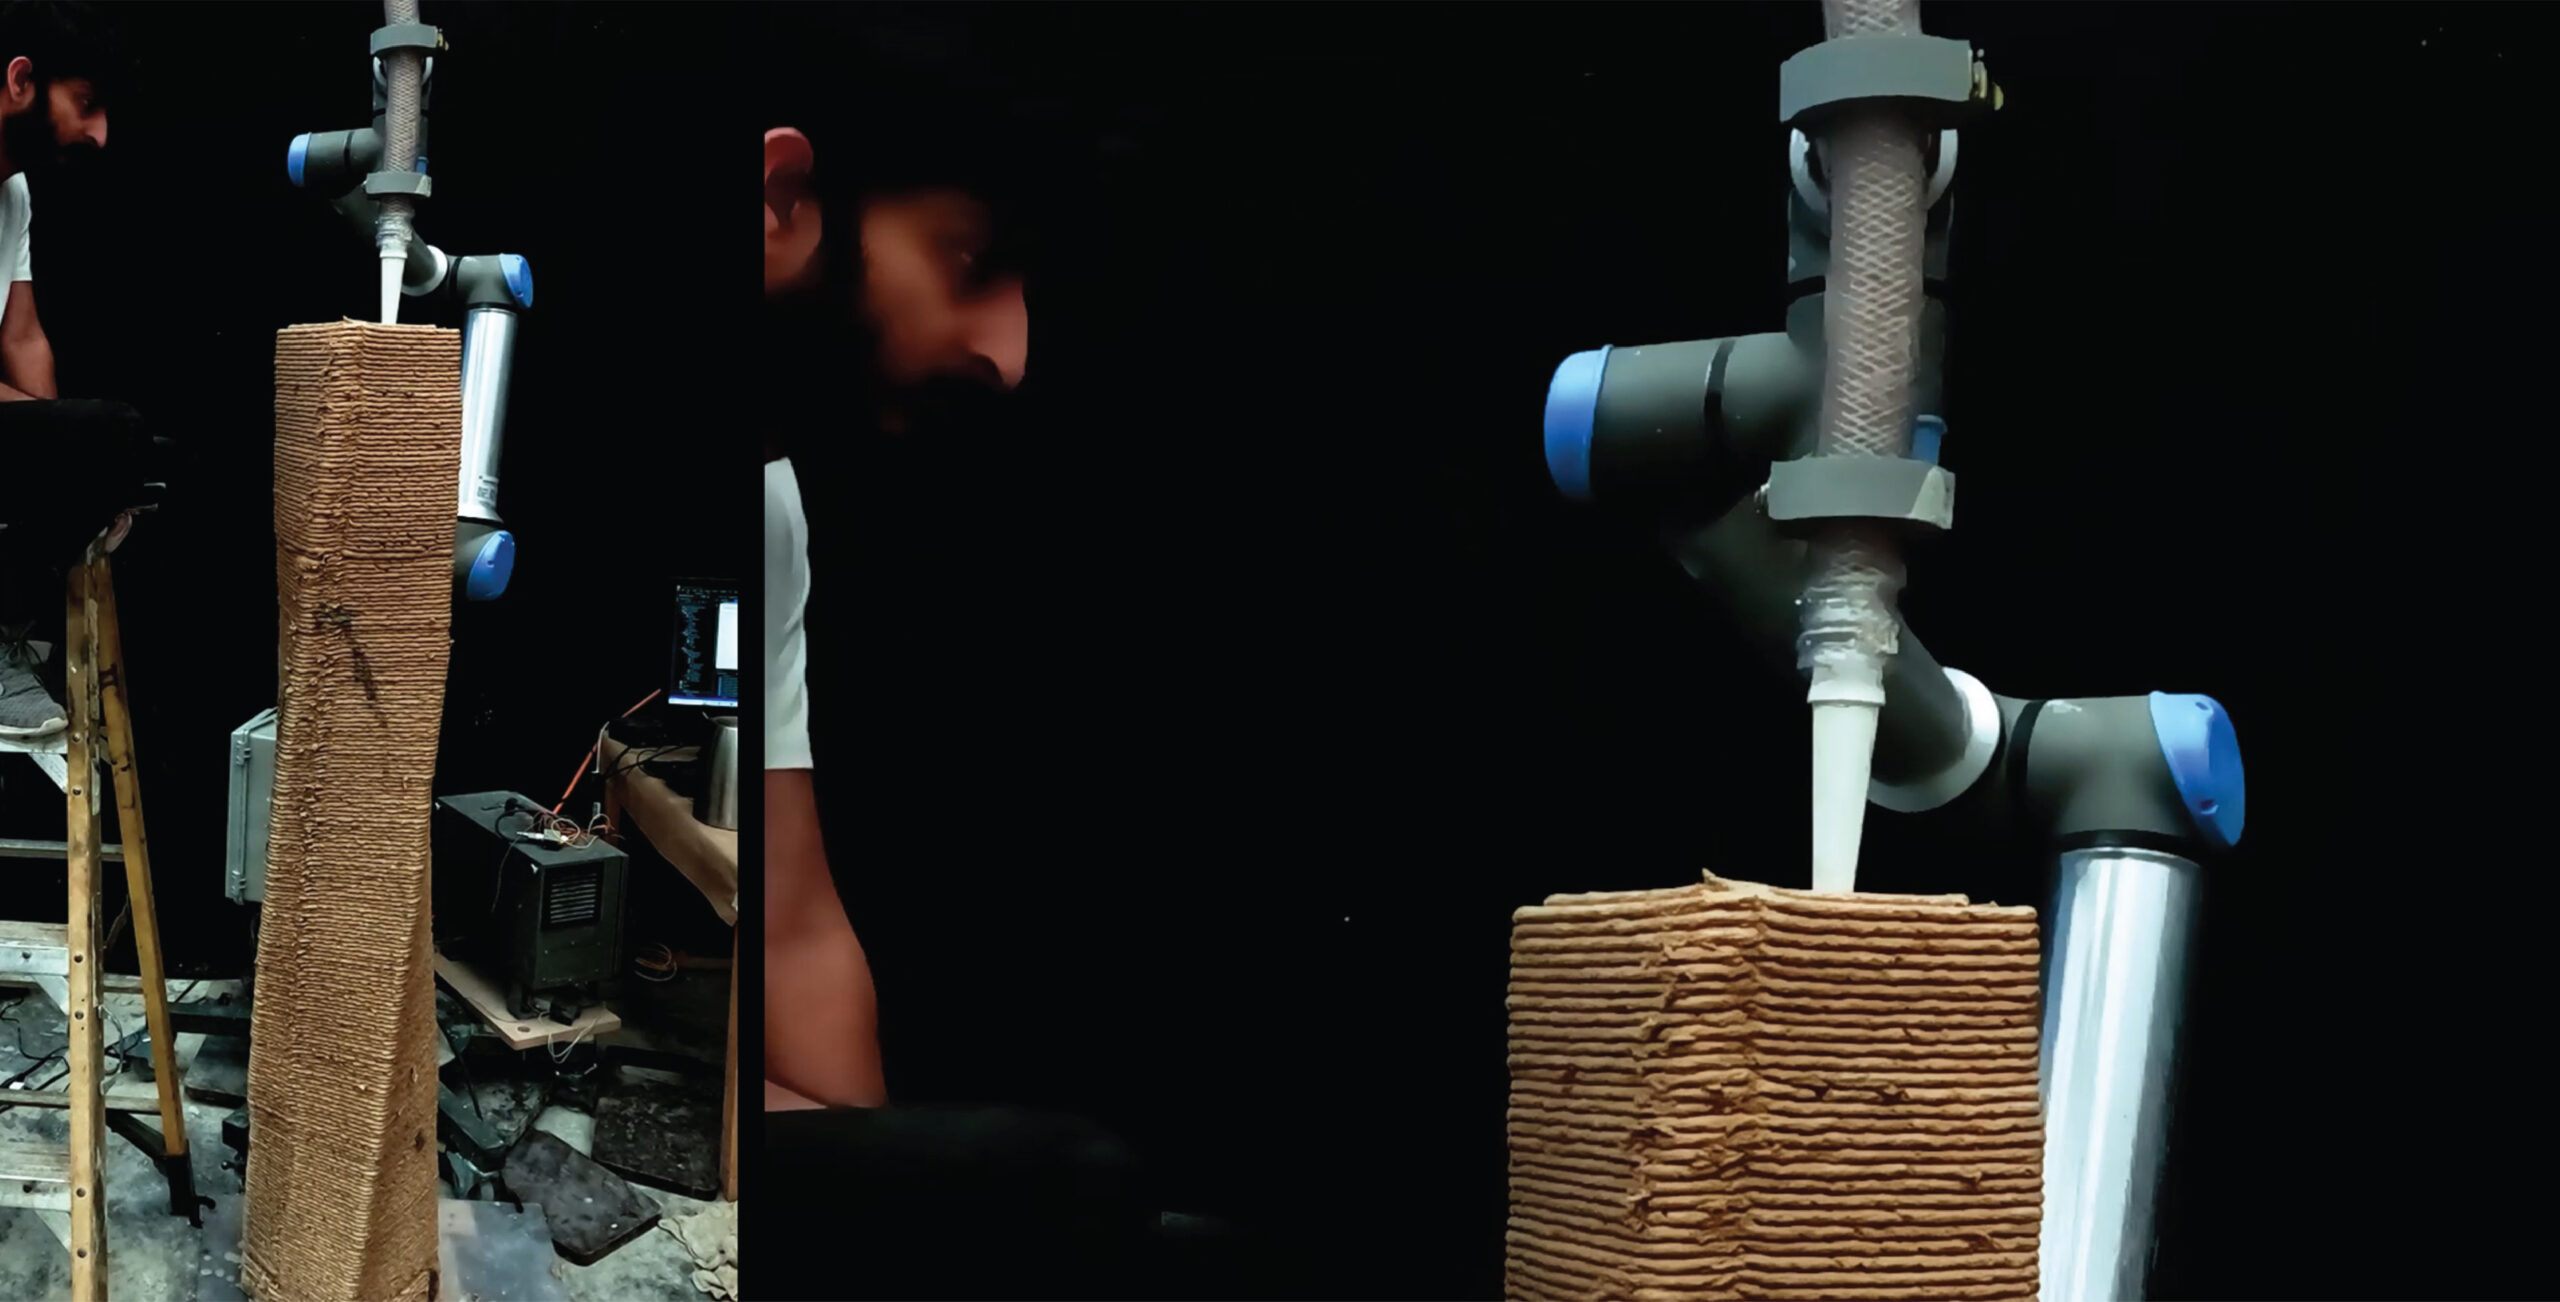
\includegraphics[width=\linewidth]{figures/beispiele/kahn-2023-2.jpg}
       \caption{\parencite{kahn2023}}
           \label{fig:kahn-2}
        \end{minipage}
    \end{figure}
\end{frame}


\begin{frame}{FDM und Optimierung f\"ur Produktdesign}
   \begin{figure}[H]
       \begin{minipage}{0.6\textwidth}
           \centering
           \vfill
           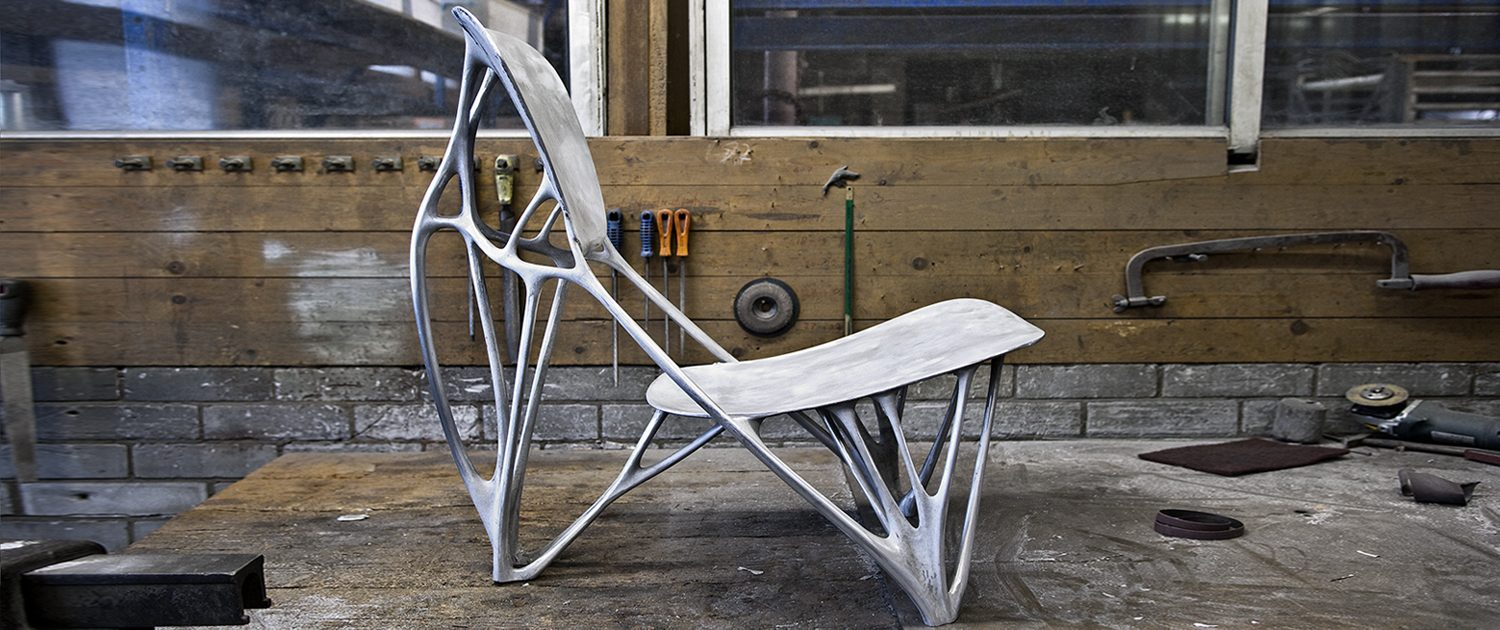
\includegraphics[width=\linewidth]{figures/beispiele/stals-2.jpg}
           \caption{Bone Chair \parencite{laarman2006}}
           \label{fig:stuhl-1}
       \end{minipage}
       \hfill
       \begin{minipage}{0.3\textwidth}
           \centering
           \vfill
           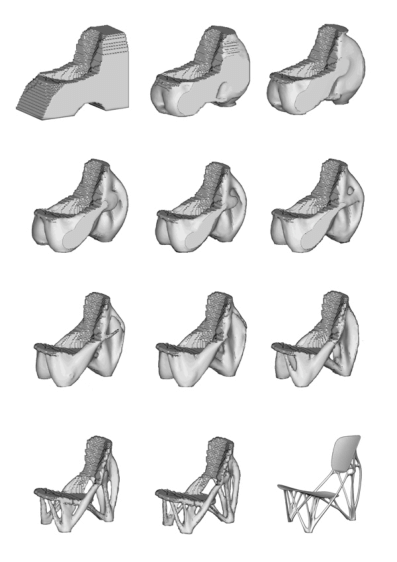
\includegraphics[width=\linewidth]{figures/beispiele/stals-1.png}
           \caption{Iterative Berechnung. \parencite{stals2015}}
           \label{fig:stuhl-2}
       \end{minipage}
    \end{figure}
\end{frame}



\section{Beispiele}
\begin{frame}{Eigenes Beipiel}
   \begin{figure}[H]
       \begin{minipage}{0.5\textwidth}
           \centering
           \vfill
           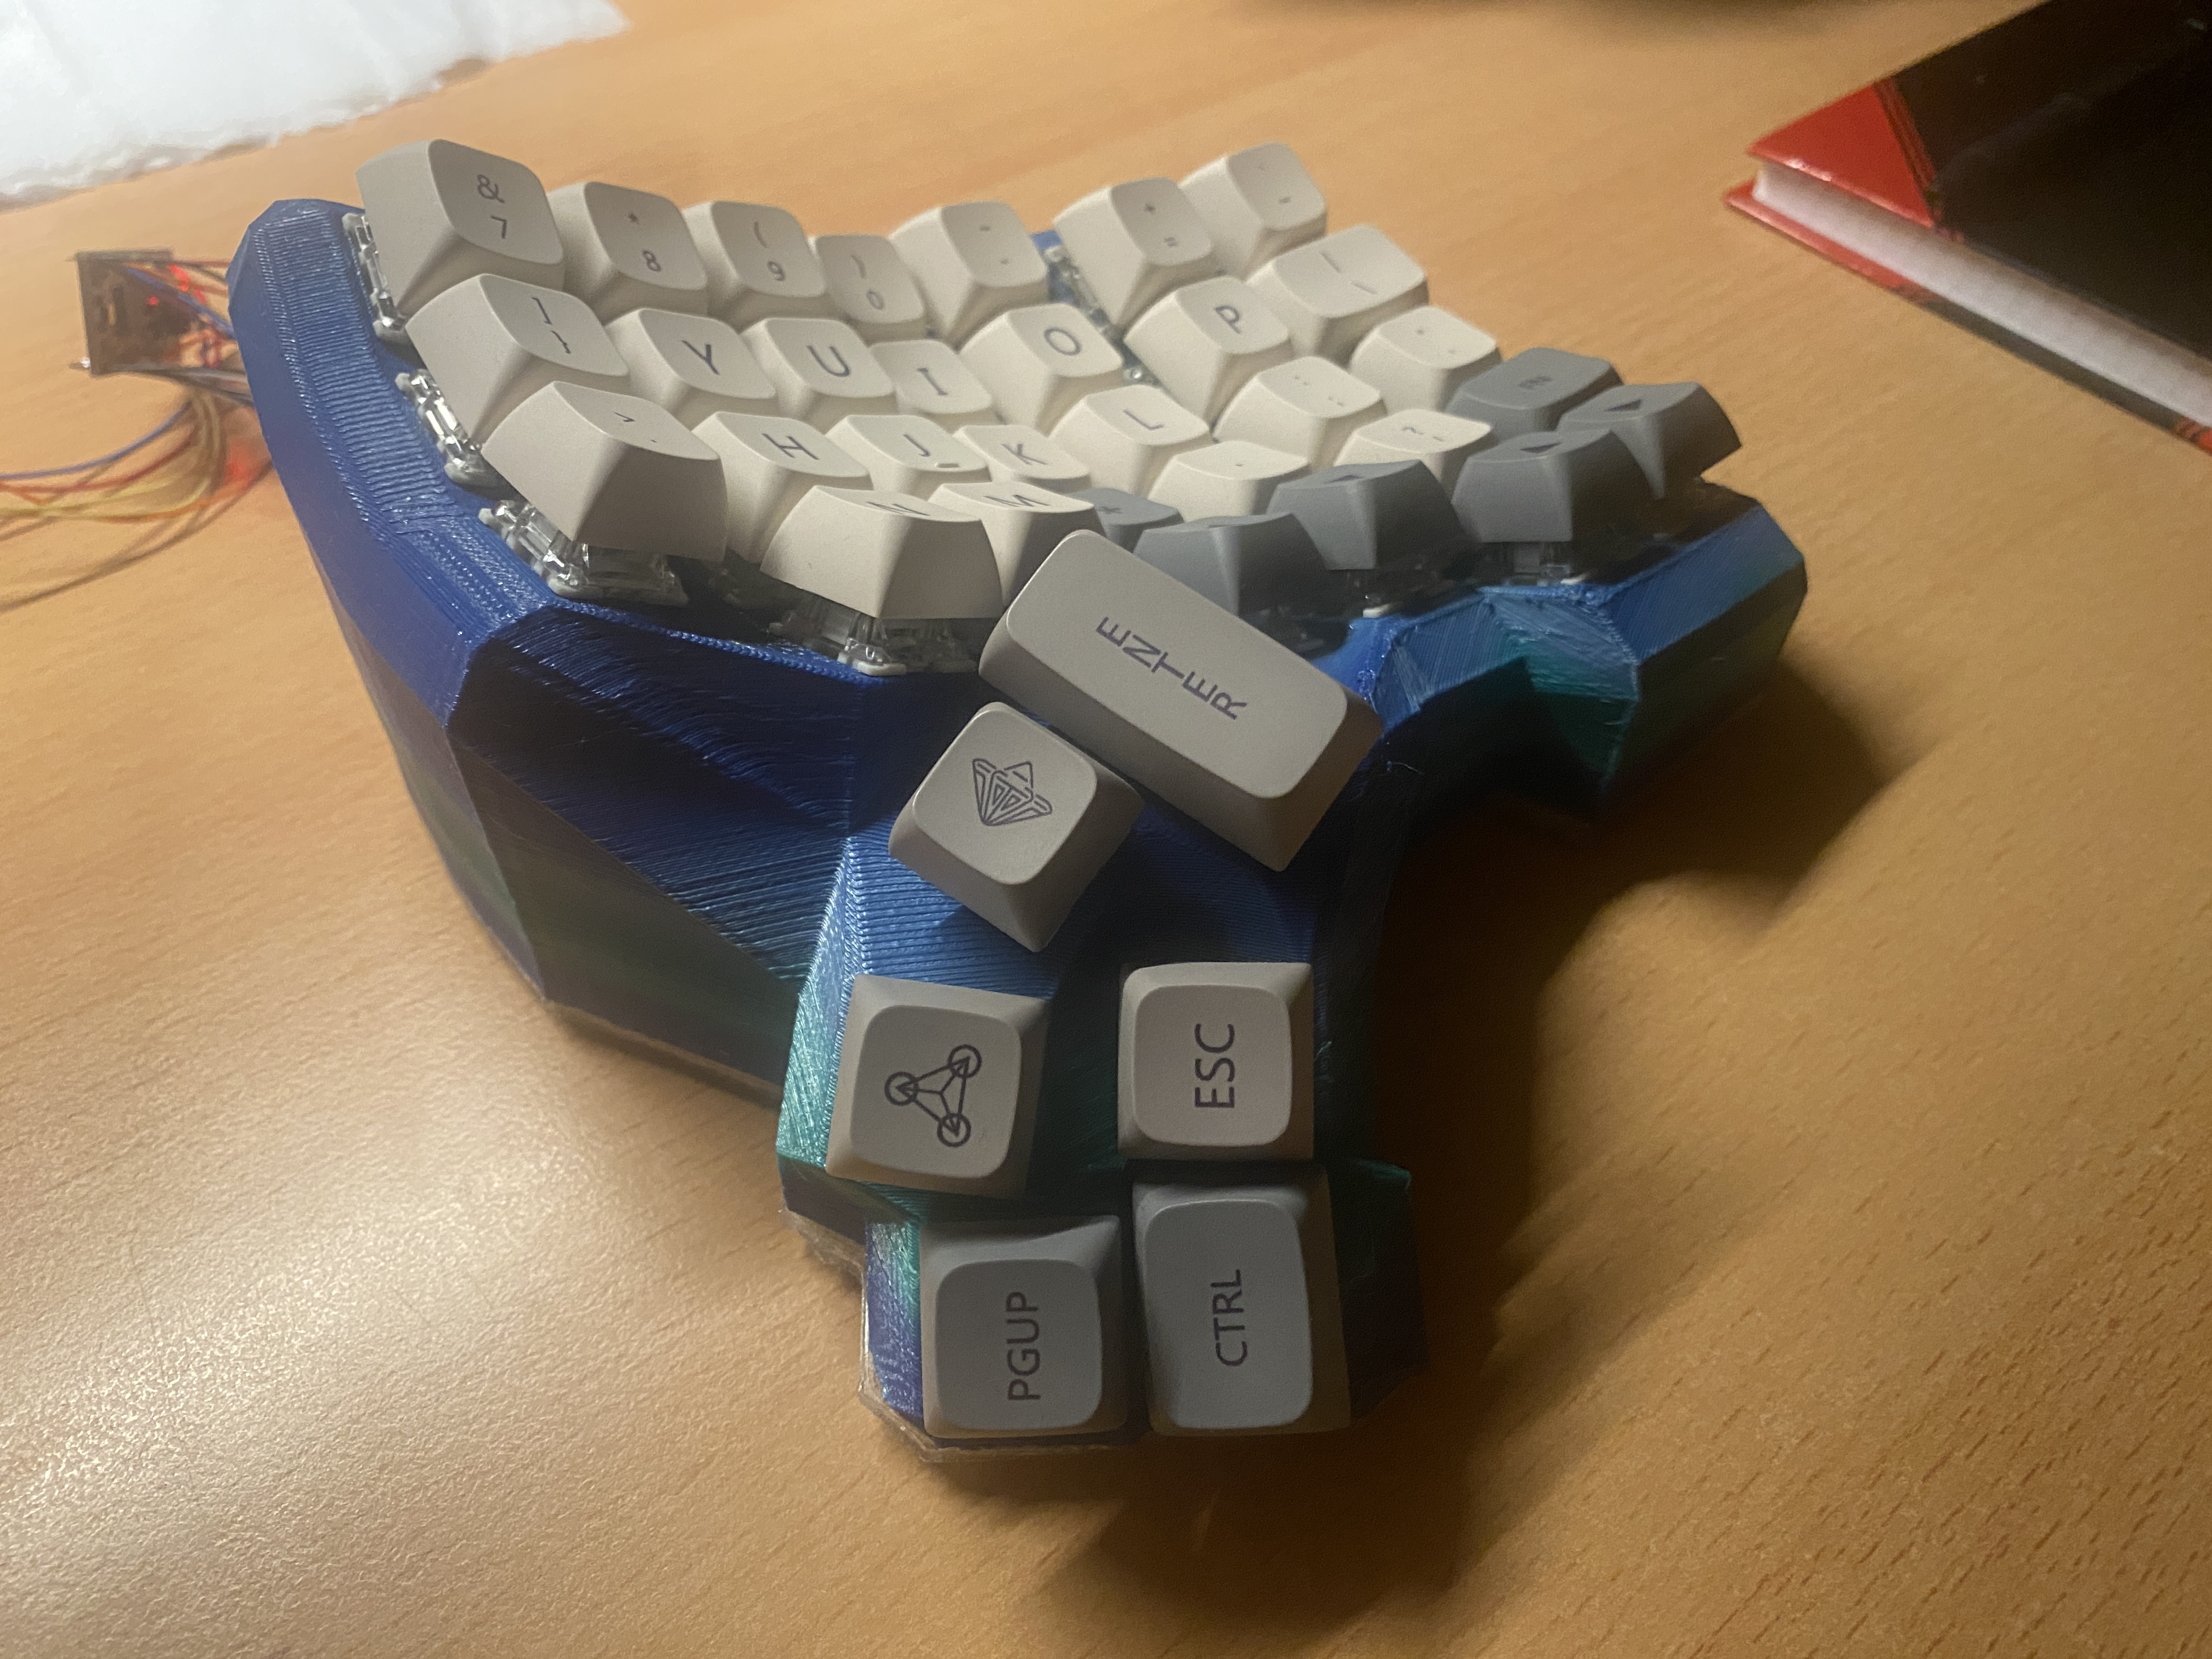
\includegraphics[width=\linewidth]{figures/dactyl.JPG}
           \caption{dactyl manuform 5x7}
       \end{minipage}
       \hfill
       \begin{minipage}{0.45\textwidth}
           Parameter:
           \begin{itemize}
               \item alle Winkel
               \item alle h\"ohen
               \item anzahl Reihen \& Spalten
               \item ...
           \end{itemize}

           Vorteile daraus:
           \begin{itemize}
               \item sehr \"Anderungsf\"ahig an alle Preferenzen
               \item Open-Source $\implies$ einfach einen fork machen wenn man eine \"Anderung will
           \end{itemize}
       \end{minipage}
    \end{figure}
    
\end{frame}



\begin{frame}{Architektur}
    \begin{figure}[H]
        \begin{minipage}{0.4\textwidth}
           \centering
           \vfill
           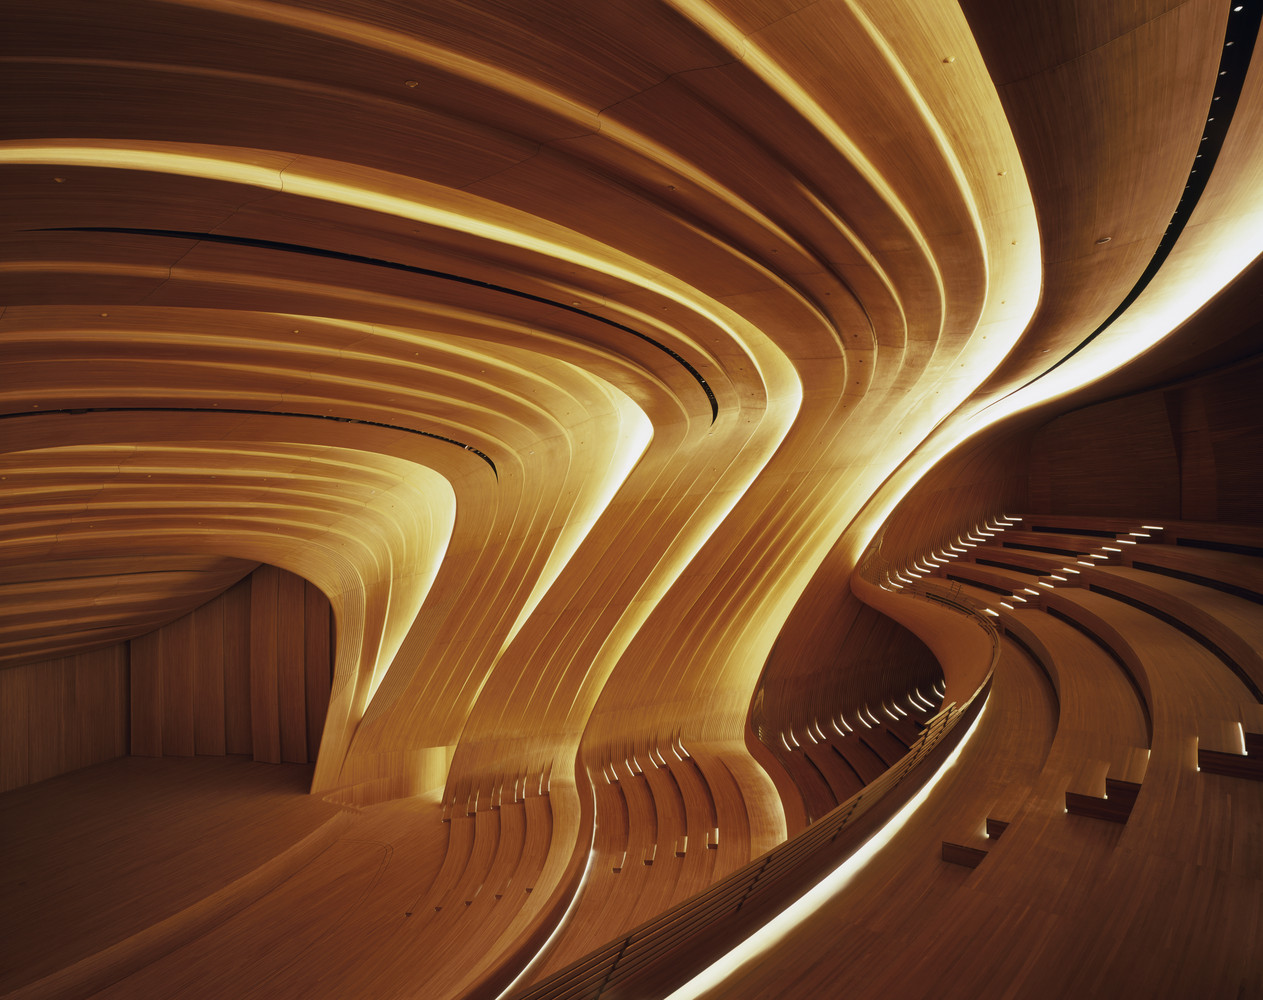
\includegraphics[width=\linewidth]{figures/beispiele/architektur/hyder-aliyev-hadid.jpg}
           \caption{Hyder Aliyev Center Azerbaijan}
           \label{fig:hadid-1}
        \end{minipage}
            \hfill
        \begin{minipage}{0.4\textwidth}
           \centering
           \vfill
           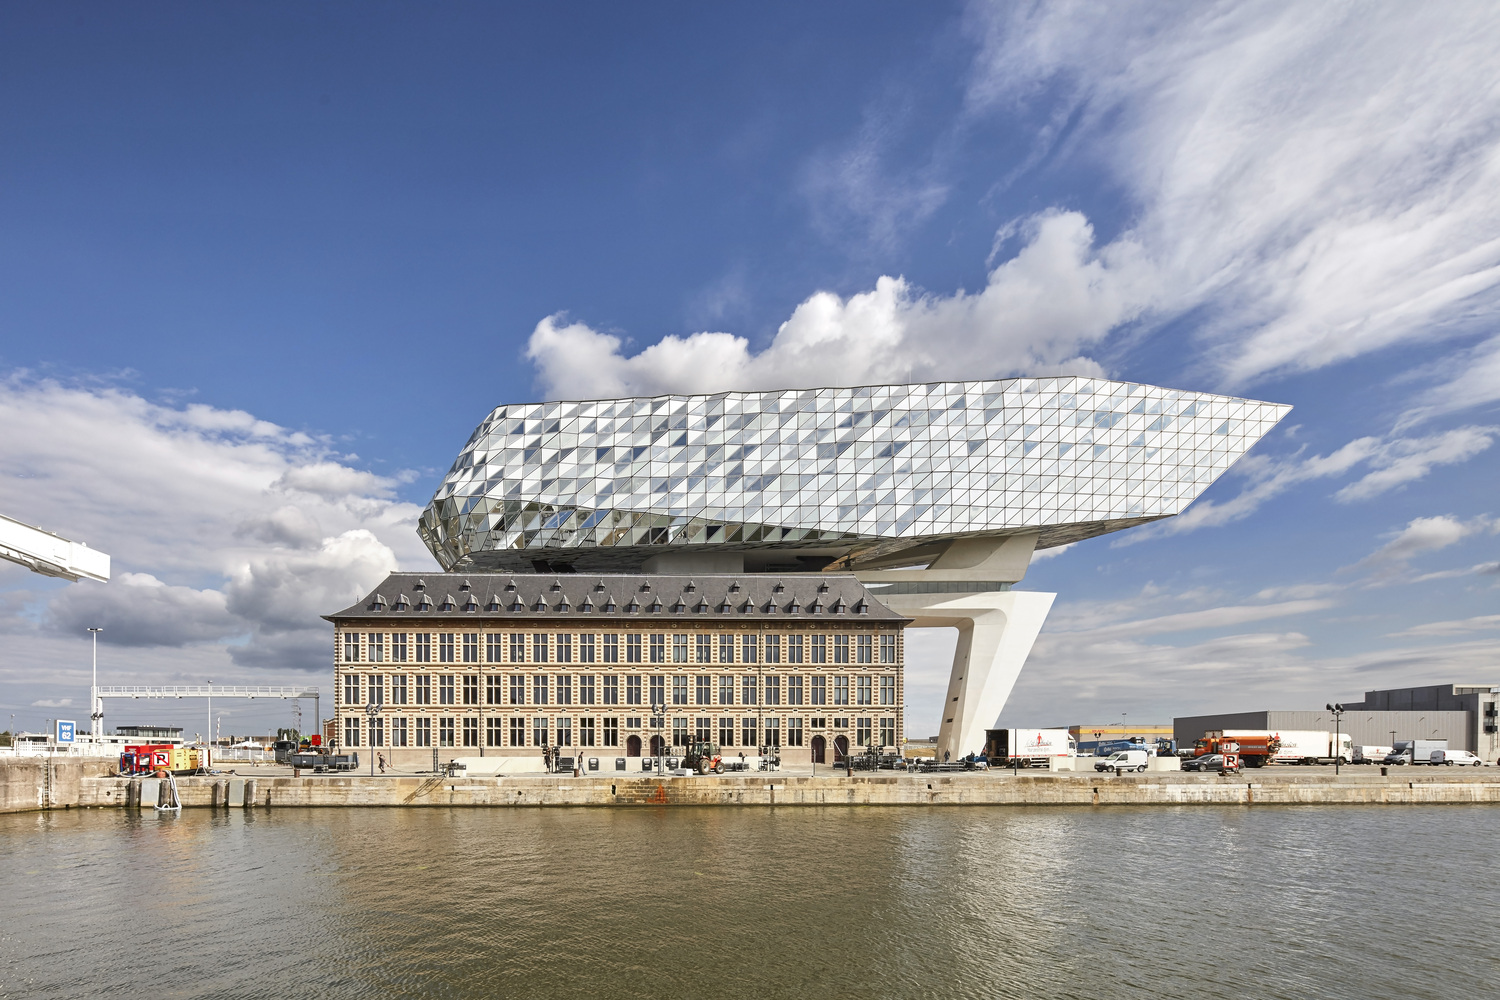
\includegraphics[width=\linewidth]{figures/beispiele/architektur/antwep-port-house.jpg}
           \caption{Port House Antwerp}
           \label{fig:hadid-2}
        \end{minipage}
    \end{figure}

\end{frame}



\begin{frame}{Ingeneurswesen}
       \begin{figure}[H]
        \begin{minipage}{0.4\textwidth}
           \centering
           \vfill
           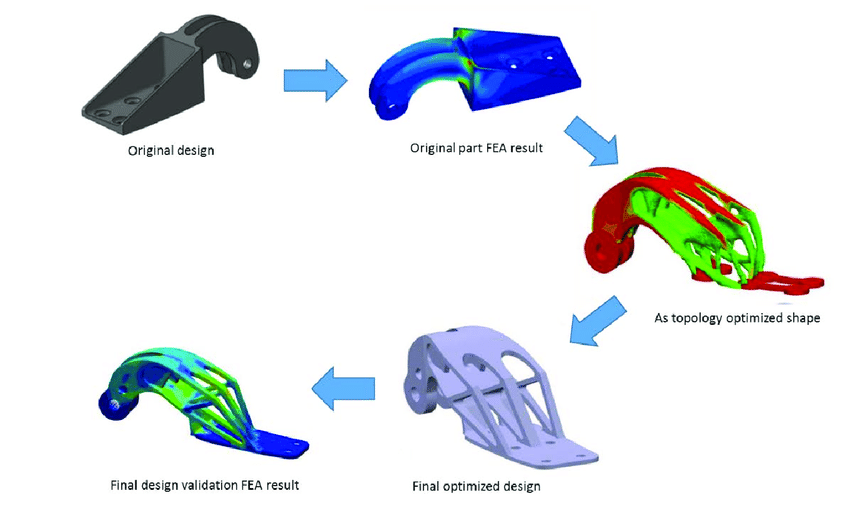
\includegraphics[width=\linewidth]{figures/beispiele/gebisa-topo-workflow.png}
           \caption{Workflow mit Parametrischem Design \parencite{gebisa2017}.}
           \label{fig:ing-1}
        \end{minipage}
            \hfill
        \begin{minipage}{0.4\textwidth}
           \centering
           \vfill
           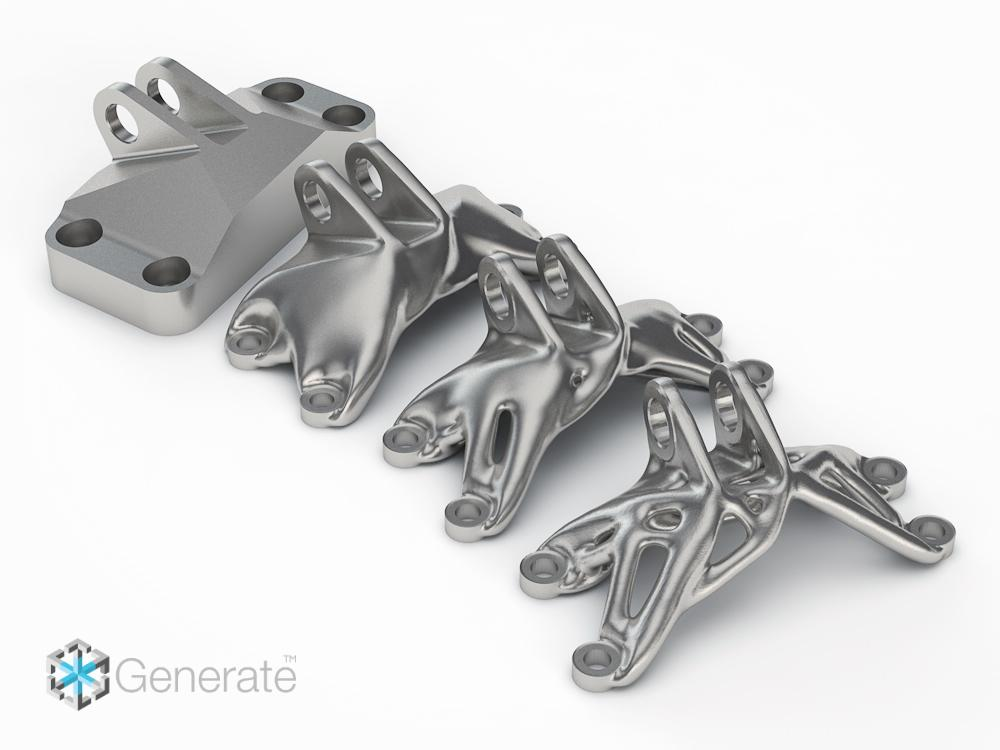
\includegraphics[width=\linewidth]{figures/beispiele/topo-ingeneur-2.jpg}
           \caption{Iterative Berechnung.}
           \label{fig:ing-2}
        \end{minipage}
    \end{figure} 
\end{frame}

\section{Tutorial}
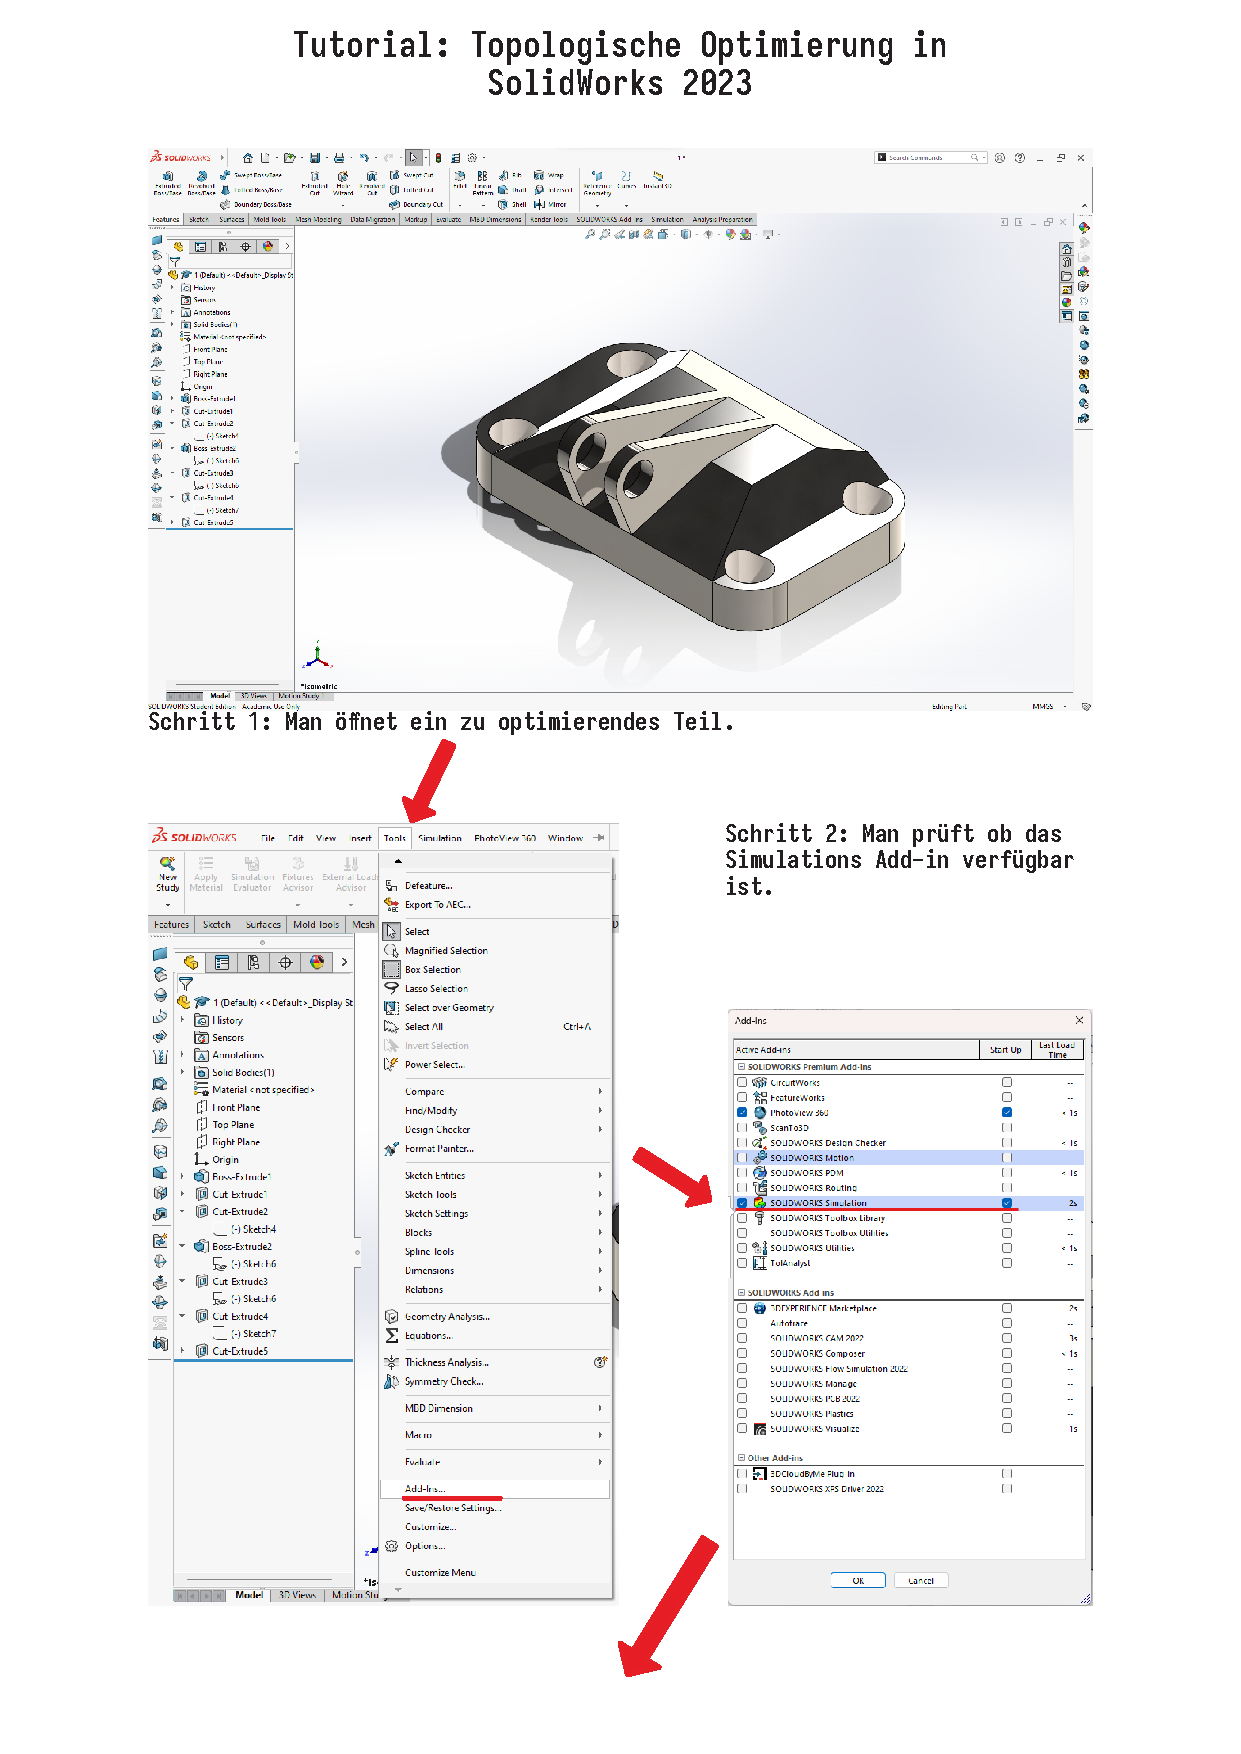
\includepdf[pages=-]{tutorial.pdf}
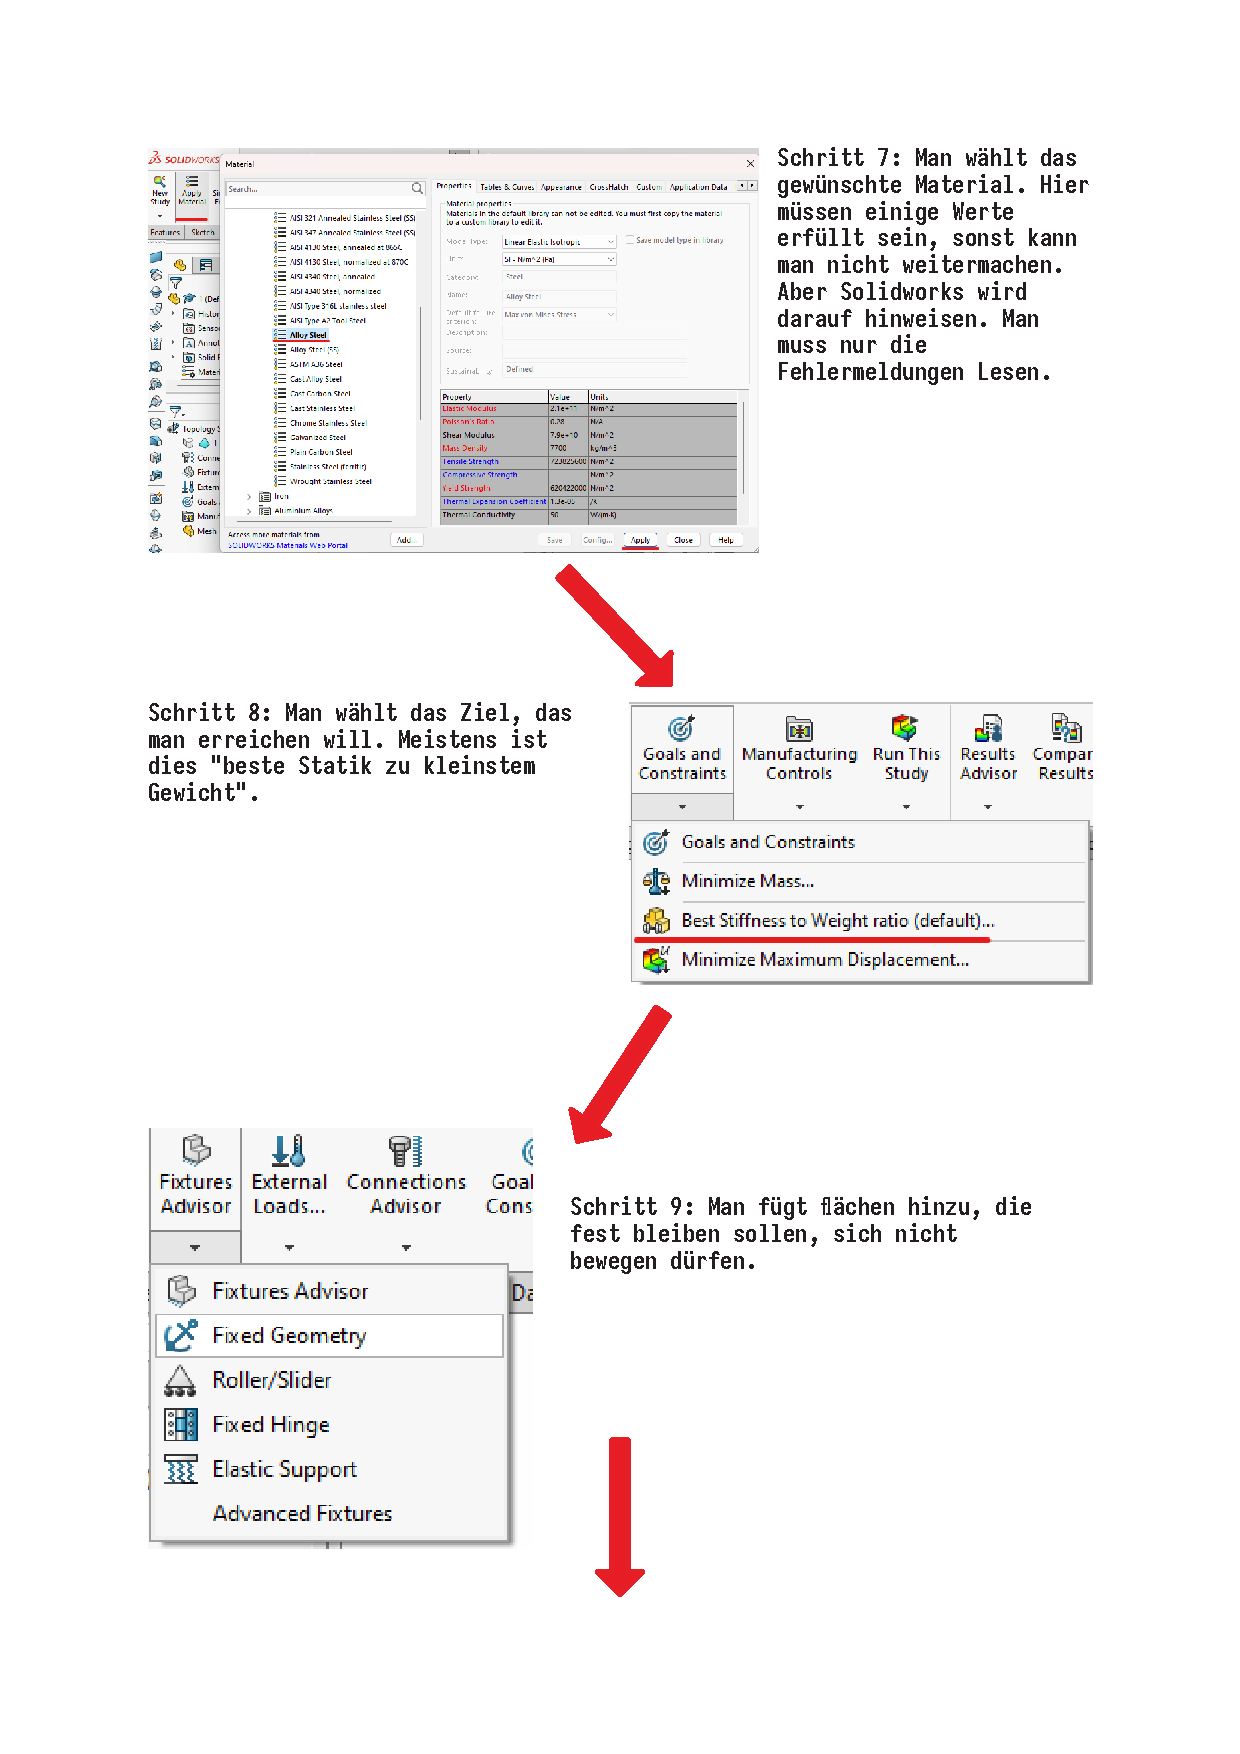
\includepdf[pages=-]{tutorial2.pdf}
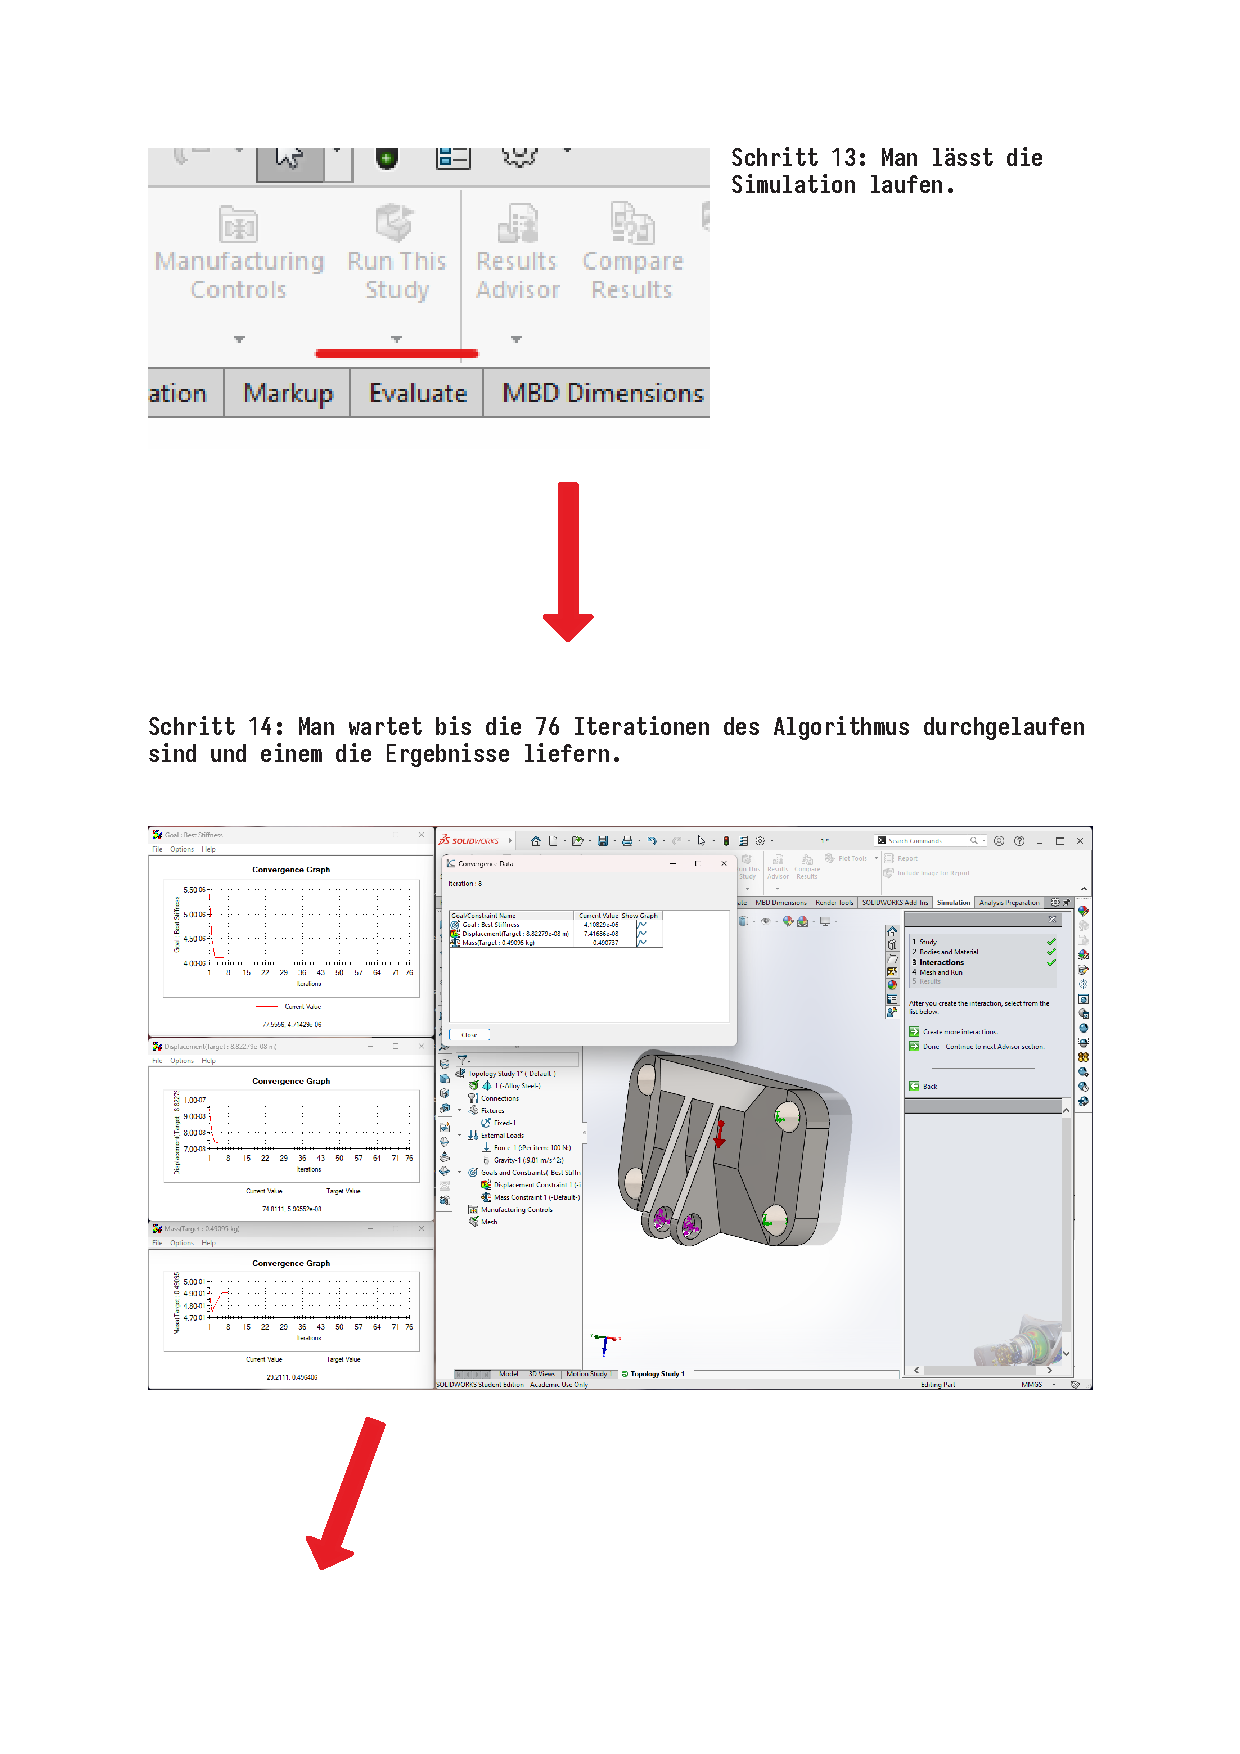
\includepdf[pages=-]{tutorial3.pdf}

\section{Andere Programme}
\begin{frame}{Rhino}
       \begin{figure}[htpb]
        \centering
        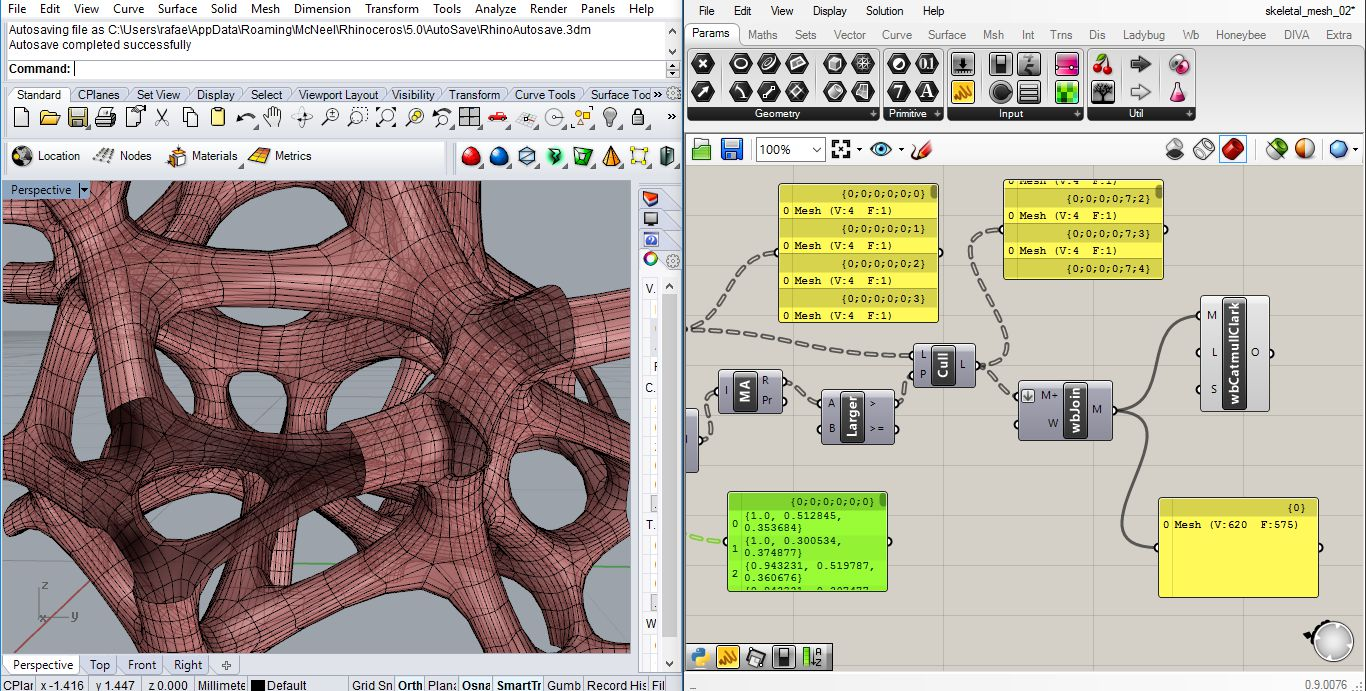
\includegraphics[width=0.8\textwidth]{figures/software/rhino.jpg}
        \caption{RhinoCAD Beispiel}
        \label{fig:rhino}
    \end{figure} 
\end{frame}

\begin{frame}{Fusion360}
   
    \begin{figure}[H]
        \centering
        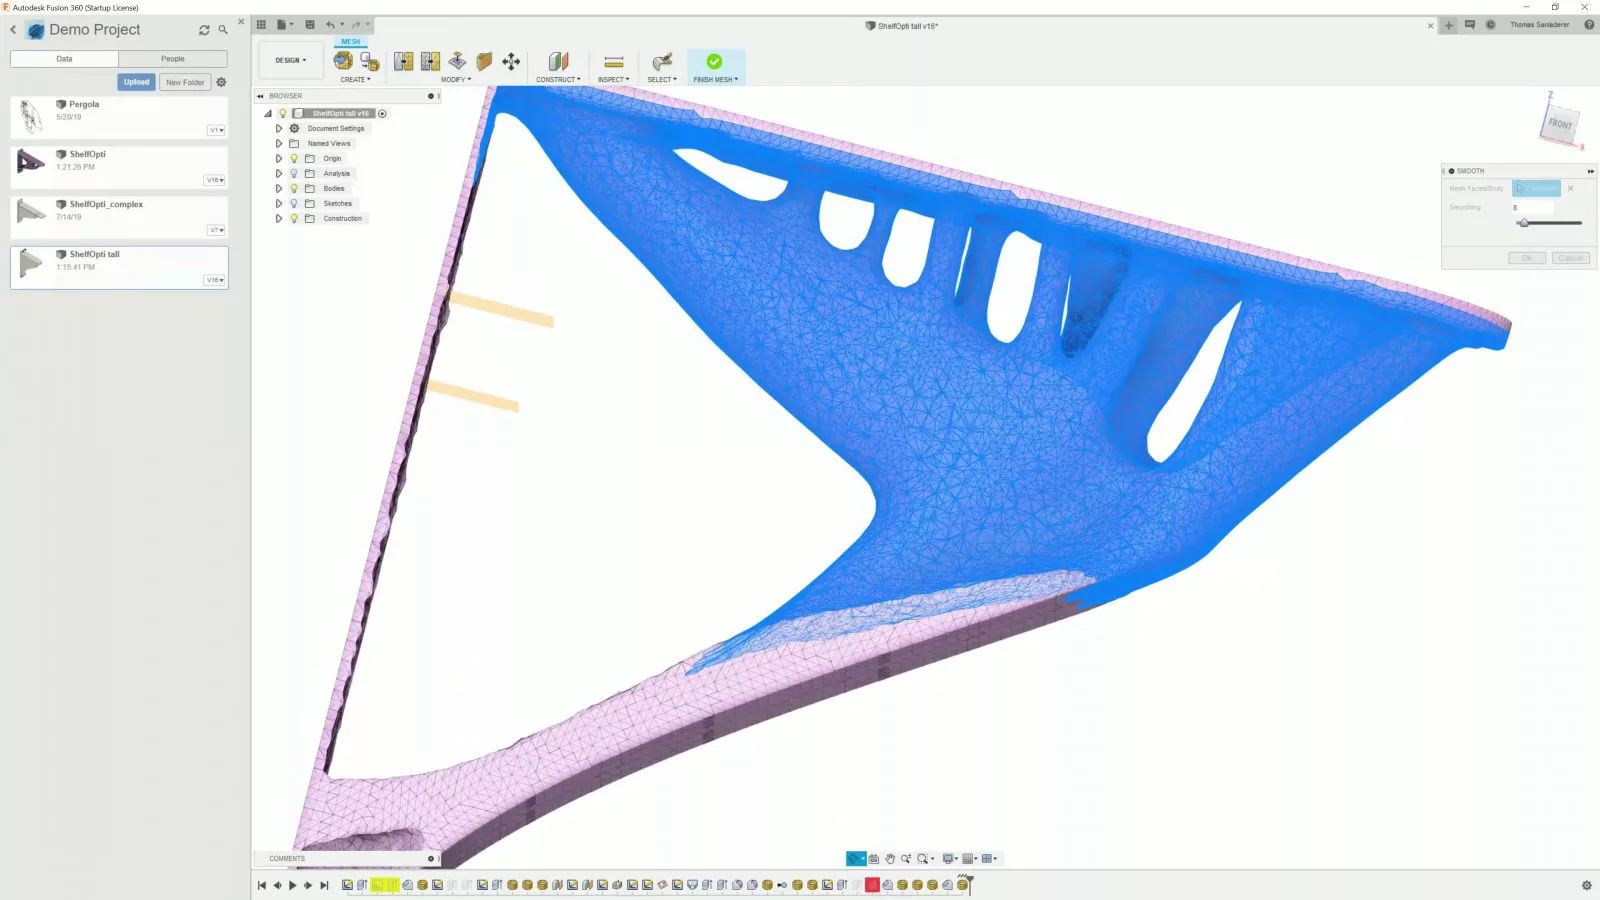
\includegraphics[width=0.8\textwidth]{figures/software/fusion.jpg}
        \caption{Fusion360 Beispiel}
        \label{fig:fusion}
    \end{figure} 
\end{frame}



\begin{frame}[allowframebreaks]{Literatur}
    \section{Ende}
    \printbibliography
\end{frame}

\end{document}
